%%% ----------------------------------------------------------
%%% Vorlage Abschlussarbeit (LaTeX)
%%% 
%%% 03/2017, Prof. Dr. Stefan Etschberger (HSA)
%%% ----------------------------------------------------------
\documentclass[12pt,a4paper,%
	             twoside,   % Fuer Veröffentlichung
	             openright, % Kapitel immer auf 
               titlepage,
               DIV12,
               pagesize=dvips,%
               headinclude,
               footinclude=false,%
               cleardoublepage=empty,%
               parskip=half,      % typographisch
                                  % besser mit Einzug,
               %pointednumbers,   % das macht die
                                  % Komaautomatik 
                                  % dudenkonform
               %draft%
               ]{scrbook}

\usepackage{blindtext}

\usepackage{Stil_Abschlussarbeit}

\usepackage[all]{nowidow}

% Literaturdatenbank
\bibliography{Literatur_Abschlussarbeit}

\usepackage{tikz}
\usepackage{xcolor}
\usepackage[colorlinks=true, 
            linkcolor=blue!60!black,
            citecolor=blue!80!black]{hyperref}

\graphicspath{{Bilder/}}

\usepackage{caption}
\DeclareCaptionLabelFormat{something}{#2.#1.}
\captionsetup[lstlisting]{labelformat=something}

\usepackage{multirow}
\usepackage{placeins}

\usepackage{tikz-uml}

\begin{document}

\pagenumbering{roman}
\setcounter{page}{1}

%%% --------------------------------------------------
%%% Titelseite
%%% --------------------------------------------------
\begin{titlepage}
%\title{
{

\begin{figure}[h]

\includegraphics[width=(0.4\textwidth)]{Bilder/ITM-Weblogo.png}
\end{figure}
\vfill

\large \sffamily
{\centering\begin{tabular}{c} \toprule
\LARGE Robotische Automatisierung im Skills Lab \\
\large Robotic Automatation in Skills Labs \\ 
\bottomrule
\end{tabular}\par}
\vspace{12ex}
\large%

\noindent
\textbf{Bachelorarbeit}\\[3ex]
im Rahmen des Studiengangs\\
\textbf{Robotik und Autonome Systeme}\\
der Universität zu Lübeck\\[6ex]

vorgelegt von\\
\textbf{Eike Schultz}\\[3ex]
Ausgegeben und betreut von\\
\textbf{Prof. Dr.-Ing. Andreas Schrader}\\[6ex]

Lübeck, den 11. März 2022
}
\end{titlepage}
%}
%\author{
%\maketitle

\chapter*{Erklärung}

Ich versichere an Eides statt, die vorliegende Arbeit selbstständig und nur unter Benutzung der angegebenen Hilfsmittel angefertigt zu haben.
\vfill
\hline

%\include{0Abstract}
%\include{03Danksagung}
\tableofcontents


%%% --------------------------------------------------
%%% real content
%%% --------------------------------------------------
\clearemptydoublepage\cleardoubleemptypage
\setcounter{page}{1}
\pagenumbering{arabic}

\addtocounter{chapter}{1}
\part{Einleitung\label{Einleitung}}
\section{Hintergrund}

In vielen Krankenhäusern ist es inzwischen üblich, Prozesse zu automatisieren und die Logistik in Teilen intelligenten Systemen zu überlassen. Dies spiegelt sich jedoch nicht in der Lehre wieder, wo eine breite Palette von Fähigkeiten erlernt werden soll. Gerade in Skills Labs, in denen Abläufe anhand von Simulationen geübt werden, findet sich ein sehr geringer Grad der Automation. Dies führt dazu, dass Simulationen entweder mit einem großen Aufwand für den Aufbau verbunden sind oder nur sehr wenige verschiedene Szenarien dargestellt werden, um den begleitenden Aufwand zu minimieren.

Die meisten Arbeiten bei der Vorbereitung von Simulationsräumen können heutzutage aber in der Praxis von Robotern und Computern erledigt werden. Dazu zählt insbesondere der Aufbau der Simulation, die Verwaltung und das Auffüllen von Verbrauchsgegenständen und die Vorbereitung der Räume selbst. Dabei ist automatische Lagerverwaltung ein weit erforschtes Feld, genauso wie der Transport von Waren in Gebäuden und der Aufbau von vorgefertigten Bauteilen. Auch die Warenwirtschaft ist heutzutage in Unternehmen standardmäßig automatisiert.

Durch eine Reduzierung des Arbeitsaufwands dieser Aufgaben kann Lehrenden mehr Zeit für die tatsächliche Lehre zur Verfügung gestellt werden. Auch bietet eine Automation die Möglichkeit, die Qualität der Lehre zu erhöhen. Dadurch, dass die Vorbereitungszeit verringert wird, können aufwendigere Simulationen durchgeführt werden oder das vorhandene Angebot um eine breitere Spanne von Simulationen erweitert werden.


\section{Zielsetzung}

Forschungsaufgabe dieser Bachelorarbeit ist es, ein Konzept für ein umfassendes Automatisierungssystem in einem Skills Lab zu entwickeln. Das System soll in der Lage sein, Lagerbestände zu verwalten und Simulationen aufzubauen, ohne dass Lehrende daran mitwirken müssen. Es soll von den Lehrenden benutzt werden können, um die Arbeit in Skills Labs zu vereinfachen und Aufgaben an das System delegieren zu können.

Dafür sollen Anwendungsfälle identifiziert werden, in denen ein solches System zum Einsatz kommen könnte, um Anforderungen zu erarbeiten, die das System erfüllen muss. Daraus soll ein Konzept erarbeitet werden, das diese Anforderungen erfüllt und in der Praxis umgesetzt werden kann.


\newpage \section{Methodik}

Um dieses Ziel zu erreichen, wird zunächst eine Analyse des derzeitigen Stands der Technik durchgeführt. Hier wird eine Literaturrecherche durchgeführt, welche Forschungsansätze und bestehende Systeme zusammenträgt. Dazu werden die Bereiche Schwarmrobotik, Lagerlogistik, Krankenhausrobotik und Mensch-Roboter Umgebungen betrachtet. Diese Recherche wird als Einstiegspunkt in die Konzeption verwendet.

Zusätzlich finden Experten-Interviews statt, um die Anwendungsfälle zu identifizieren. Diese Interviews finden mit Verantwortlichen für die existierenden Skills Labs der Universität zu Lübeck sowie anderer Einrichtungen statt. Aus diesen Interviews werden funktionale Anforderungen an das System gestellt, die es zu erfüllen gilt. Auch werden dabei mögliche Feature-Sets sondiert, welche das System erweitern können, um einen größeren Mehrwert zu bieten.

Im Anschluss wird ein Konzept erarbeitet, welches den gestellten Anforderungen gerecht wird. Dazu werden die benötigten Komponenten des Systems erarbeitet und in eine gemeinsame Systemarchitektur integriert. Dieses Konzept wird dann in einer Implementierung realisiert, um die Umsetzbarkeit zu beweisen. Zur Erbringung des Beweises wird eine Evaluation der Implementierung durchgeführt.

In einer anschließenden Diskussion wird schließlich das realisierte Konzept mit den Anforderungen verglichen und ein weiterer Wegplan für das System aufgezeigt. Dies umfasst das Erfassen einer Aufwandsabschätzung und der technischen Voraussetzung und Herausforderungen einer Implementierung.
\setcounter{section}{0}

\addtocounter{chapter}{1}
\part{Analyse\label{Analyse}}
\section{State of the Art}

In Vorbereitung auf die Konzeptionierung wurden aktuelle wissenschaftliche Arbeiten untersucht, um ähnliche Ideen zusammenzutragen und auf diesen aufzubauen. Da in der Automatisierung optimale Strategien von den lokalen Gegebenheiten abhängen und es keine allgemein gültigen Lösungen für alle Arbeitsbereiche gibt, werden zunächst verschiedene Lösungsansätze für Teilprobleme der Aufgabe betrachtet. Aufbauend auf diesen werden dann im weiteren Verlauf dieser Arbeit Ansatzpunkte gewählt, die eine Lösung für die Forschungsfrage ermöglichen.

Hierfür wurden die beiden Themenkomplexe der Schwarmrobotik und Lagerlogistik besonders betrachtet, da eine Automatisierung in Skills Labs durch eine Gruppe von autonomen mobilen Robotern besonders auf diesen aufbaut. Die Schwarmrobotik beschäftigt sich mit der Interaktion zwischen und der Organisation von einer größeren Menge Robotern in einer gemeinsamen Umgebung. Die Lagerlogistik dagegen beschreibt die Organisation einer möglichst effizienten Lagerverwaltung, welche in den letzten Jahren durch das Aufkommen von mobilen Roboterplattformen stark verändert wurde.

Zudem wurden mehrere Themenkomplexe betrachtet, die in Teilaufgaben der Automatisierung von Skills Labs mit einfließen. Dazu zählen insbesondere die Krankenhausrobotik, also die Verwendung von robotischer Unterstützung in Krankenhausabläufen, sowie die Robotik in Umgebungen, die gemeinsam mit Menschen genutzt werden.

Das Ziel der Schwarmrobotik ist, dass sich verschiedene Roboter in einer gemeinsamen Umgebung nicht gegenseitig behindern und bestenfalls sogar zusammenarbeiten, um gemeinsame Ziele zu erreichen. Ein zentraler Forschungsschwerpunkt ist dabei derzeit, einen Grat zwischen Performanz, Robustheit in einer komplexen Umgebung und Skalierbarkeit der verwendeten Roboter-Anzahl zu schlagen. Die sinnvolle Steuerung eines Roboters anhand von Sensordaten in Echtzeit ist eine Aufgabe, die eine nicht vernachlässigbare Menge Rechenaufwand erfordert. Dementsprechend ist ein System, das eine größere Anzahl von Robotern gleichzeitig steuert, aufwendig zu implementieren und Gegenstand der aktuellen Forschung.

Die Arbeit von Inoue et al. \cite{meanField} beispielsweise versucht dieses Problem zu lösen, indem einzelne Roboter als Partikel in einem Mean-Field Game betrachtet werden. Das bedeutet, dass der explizite Zustand einzelner Roboter nicht vom Kontrollsystem erfragt und ausgewertet wird, sondern anhand der physischen Position geschätzt wird. So ein Ansatz ermöglicht es, große Mengen Roboter anzusteuern, ohne eine lineare Skalierung des Rechenaufwands zu erzeugen. Dies geht zulasten der Qualität der einzelnen Steuerungsanweisungen, daher war der Forschungsschwerpunkt der Arbeit, den Fehler zwischen der Schätzung und dem tatsächlichen Zustand der eingesetzten Roboter zu minimieren. Ein solches System setzt voraus, dass es eine große Anzahl von Robotern gleicher Bauart gibt, über die die zentrale Steuerung mitteln kann.

Einen Ansatz, diese Beschränkung zu umgehen, liefert die Arbeit von Olcay et al. \cite{collectiveNav}. Anstatt eine Steuerung vorzugeben, teilen die einzelnen Roboter mit der zentralen Kontrolleinheit ihre Sensordaten, welche diese zu einem gemeinsamen Weltmodell zusammenführt und an alle Roboter zurück gibt. Dadurch soll den einzelnen Robotern ermöglicht werden, bessere Entscheidungen in der eigenen Navigation zu treffen. So kann auch eine kollektive Bewegungsplanung ermöglicht werden, in der sich die Roboter nicht im Weg stehen, obwohl die Roboter völlig autonom handeln. Da dies nicht voraussetzt, dass die einzelnen Agenten identisch sind, sondern nur ein gemeinsames Weltmodell verstehen, kann eine Vielzahl verschiedener Modelle verwendet werden.

Diese beiden Ansätze setzen voraus, dass alle Roboter die gesamte Einsatzzeit mit einem zentralen Server verbunden sind. In der Praxis kann dies aber nicht immer gewährleistet werden. Andere Forschungsgruppen setzen daher auf dezentrale Steuerungsmodelle. Das hat den Vorteil, dass das System robust gegenüber Kommunikationsausfällen ist und weniger Datenaustausch erfolgen muss.

Im Ansatz von Fan et al. \cite{mlTrain} wird daher versucht, einzelnen Robotern ein kooperatives Verhalten beizubringen. Anstatt während der Laufzeit mittels fortlaufender Kommunikation Entscheidungen zu treffen, werden die Roboter mittels maschinellen Lernens für entsprechende Situationen trainiert. Dies muss nicht in einer physischen Umgebung passieren, sondern kann in einer Simulation vor dem Einsatz stattfinden. In dieser lernen die Roboter, einander möglichst effizient auszuweichen und Kollisionen zu vermeiden, um dies dann auch zur Laufzeit zu tun. Dadurch kann die zentrale Steuerung sich darauf beschränken, grobe Anweisungen wie Zielpunkte vorzugeben, während das explizite Verhalten in verschiedenen Situationen den Robotern selbst überlassen wird. Die Arbeit zeigt, dass solch ein Ansatz sowohl robust gegenüber Änderungen in der physischen Form des Roboters ist, wie sie im Transport von Möbeln auftreten würden, als auch gegenüber der Anwesenheit von Menschen in derselben Umgebung. Der Nachteil hiervon ist aber, dass das maschinelle Lernen der Steuerung von Robotern aufwendig ist und sich bei drastischen Änderungen der Umgebung wiederholt.

Die Arbeit von Reily et al. \cite{silentSwarm} setzt statt auf ein vorheriges Trainieren der Roboter daher darauf, dass jeder einzelne Roboter nicht nur den eigenen Pfad planen kann, sondern genauso den anderer ihm bekannter Roboter. Hier werden mögliche Kollisionen vermieden, indem jeder Roboter die Position anderer Roboter in seinem Weltmodell bestimmt und anhand deren bekannten Zielkoordinaten einen idealen Pfad berechnet. 

Dabei wird auf die Spieltheorie zurückgegriffen, um ein insgesamt besseres Ergebnis zu erzielen, indem jeder Roboter sich kooperativ verhält. Dabei werden neben dem Abstand des Roboters von seinem Ziel auch der zu anderen Plattformen und Hindernissen als zu berücksichtigende Parameter der Wegplanung miteinbezogen. Dadurch, dass jeder Roboter nicht nur versucht, einen optimalen Weg für sich selbst zu finden, sondern auch Vorhersagen über das Verhalten anderer Roboter macht, kann er einen Plan entwickeln, der für alle Roboter das optimale Ergebnis erzielt. Auf diese Art soll ein gemeinsames koordiniertes Vorgehen entstehen, ohne dass die Roboter miteinander kommunizieren oder eine zentrale Einheit die Navigation steuert.

Dies setzt voraus, dass jeder Roboter in der Lage ist, mehrere Wegplanungen gleichzeitig zu berechnen. Auch muss jeder Roboter jeden anderen im System erkennen und dessen Wegziel wissen können. Die erste Voraussetzung kann in modernen Robotern als gegeben angesehen werden, da die Wegplanung bei angemessener Optimierung nur einen Bruchteil der benötigten Rechenleistung darstellt. Um die zweite Voraussetzung zu erfüllen, müssen Roboter entweder untereinander kommunizieren können oder über ein zentrales System ihre Position mitteilen.

Die Lagerlogistik setzt bei der Automatisierung in der Regel auf einen makroskopischen Ansatz. Einer der zentralen Begriffe hier ist Robotic Mobile Fulfillment System, als RMFS abgekürzt. Er bezeichnet Systeme, bei denen Roboter den Großteil der Vorgänge in der Logistik übernehmen, anstatt diese händisch durchführen zu lassen. Die Roboter werden dabei nicht nur als Ersatz für menschliche Arbeiter verwendet, sondern sind zentraler Teil des Warenhauses.

Ein gutes Beispiel hierfür ist in der Arbeit von Keung et al. \cite{cloudFullfillment} zu finden. Die Entwicklung von Internet of Things-Geräten erlaubt es, Möbel und vormals statische Gegenstände in ein cyber-physikalisches System zu integrieren. Mittels eines zentralen Cloudservers können diese IoT-Geräte, Roboterplattformen und die Kommunikation zwischen diesen abgewickelt werden. Diese Einbindung von cyber-physikalischem System und Robotern verspricht eine Effizienzsteigerung der Abläufe, die eine reine Verwendung von nur einer der beiden Technologien nicht erreichen könnte. In dieser Arbeit wird dies über eine mehrschichtige Regelordnung erreicht, welche Aufgaben in übergeordneten Zielen, für die mehrere Systeme zusammenarbeiten müssen, sowie kleinen Aufgaben, welche von einem einzelnen System des RMFS bewältigt werden können, einordnet.

An einer solchen Aufgabenplanung hat auch das Team Bolu et al. gearbeitet \cite{adaptivePlanning}. Da RMFS sehr dynamische Umgebungen sind, die sich ständig verändern, wurde versucht, ein zentrales Aufgaben-Management zu implementieren. Damit sollen die begrenzten Ressourcen möglichst effizient genutzt werden. Das Management-System nimmt daher Daten wie den Standort von Robotern, anstehende Aufgaben und mögliche Zusammenarbeitsmöglichkeiten von Systemen auf. Aus diesen Daten erstellt es dann adaptiv Aufgaben für die einzelnen Geräte, welche ansonsten ohne Rücksicht auf die jeweilige aktuelle Situation verteilt werden würden.

Ein Ansatz zur Anpassung von Automatisierungsalgorithmen an sich ändernde Gegebenheiten ist auch in der Arbeit von Xiang et al. \cite{BIMExtension} zu finden. Die Forscher schlagen einen hybriden Ansatz vor, bei dem Algorithmen und die logistischen Gegebenheiten in Tandem optimiert werden, um besser aufeinander abgestimmt zu werden. Der vorgeschlagene Wegplanungsalgorithmus soll durch Einsatz von künstlicher Intelligenz auf Ausnahmesituationen reagieren können, indem er sich dynamisch an sich ändernde Umstände anpasst. Dies kann im Einsatz in Skills Lab auch abseits von solchen Situationen von unermesslichem Wert sein, da sich Simulationen im Aufbau und den Anforderungen stark unterscheiden können,weshalb jede Wegplanung robust gegenüber Änderungen der Arbeitsumgebung sein muss.

Andere Forschungsgruppen beschäftigen sich statt mit der Aufgabenverteilung in der Logistik mit der effizienten Pfadplanung von autonomen Roboterfahrzeugen, Automated Guided Vehicle oder AGV genannt. Die Arbeit von Zhang et al. \cite{routeAGV} beispielsweise beschäftigt sich mit der Vermeidung von Kollisionen in den Abläufen. Da automatisierte Warenhäuser möglichst wenige Flächen für die Navigation freihalten möchten, ohne die Effizienz der eingesetzten AGVs zu verringern, beschäftigte sich das Team mit der Wegplanung. Anhand der Zeitpläne der verschiedenen Arbeitsstationen im Lager werden die Wege so geplant, dass die Wartezeiten von AGVs an diesen minimiert werden. In der vorgestellten Gitter-basierten Wegplanung implementiert das Forschungsteam drei verschiedene Strategien, um die jeweiligen Planungskollisionen zu vermeiden.

Einen anderen Ansatz verfolgen Yang et al. \cite{2DPlan}. Sie implementierten die Wegplanung, indem diese als Botenproblem betrachtet wird. Die einzelnen Aufgaben im Lager werden als anzufahrende Stationen in einem statischen Gitter-Modell betrachtet. Ausgehend von einer ersten Aufgabe werden nach und nach mehr anzufahrende Stationen hinzugefügt und eine optimale Strategie für die Reihenfolge der Aufgabenerledigung gefunden. Dies erhöht die Performanz individueller AGVs gegenüber anderen Planungsarten, da optimale Pfade schneller gefunden werden.

Zur Implementierung einer solchen Strategie ist es nötig, eine Karte der Umgebung zu besitzen, in der Aufgaben wie der Ort zu transportierender Möbel und anzufahrender Ablagepunkte lokalisiert werden können. Dies ist jedoch für nahezu alle Navigationsansätze nötig, sodass es keine gesonderte Herausforderung darstellt. Der Vorteil dieses Ansatzes ist besonders bei komplexen Wegplanungen spürbar, bei denen die Berechnung signifikante Ressourcen benötigt. Dies kann im zu entwerfenden System dann auftreten, wenn Möbel aus verschiedenen Räumen zusammengetragen werden müssen oder weniger Roboter als Möbel zur Verfügung stehen, sodass die Wegfindung optimiert werden muss.

Ein wichtiger Unterschied zwischen dem Einsatz von Robotern zum Transport von Möbeln in einem Skills Lab und standardisierten Objekten in einem darauf ausgelegten Warenhaus ist die verschiedene Handhabung der Ladung. Während in einem Warenhaus die Objekte in leicht zu erreichenden Regalen gelagert sind, müssen im Skills Lab voraussichtlich sehr verschieden geformte Gegenstände vom Boden aufgehoben werden.

In der Arbeit von De La Puente et al. \cite{assistRobot} wird dieses Problem mithilfe von bereits bestehenden Robotern gelöst. Der hier vorgestellte Algorithmus ermöglicht diesen, beliebige Objekte vom Boden aufzuheben. Die Forschung baut dabei auf bereits bestehenden Projekten in Laborszenarien auf und erweitert diese auf Realbedingungen durch Einbindung aller dazu benötigten Komponenten. Diese umfassen in den Experimenten eine mobile Plattform, eine Sensoreinheit auf einem beweglichen Kopf und einen Arm mit Greifer.

Der Schwerpunkt der Arbeit liegt dabei neben der Performanz auf der Robustheit des Systems. Der Forschungserfolg liegt darin, dass der Roboter die Aufgabe in unübersichtlichen und dynamischen Umgebungen mit Menschen erfüllen kann, wie es auch in einem Skills Lab der Fall ist. Der Roboter kann dabei selbstständig anhand der Position und Größe  der Objekte feststellen, ob sie von ihm aufgehoben werden können. Da die Objektauswahl auch auf andere Weise erfolget, beispielsweise durch eindeutige Positionsangaben im 2D-Raum, und mit wenig Aufwand automatisiert werden kann, ist dies auch für einen Einsatz im Skills Lab geeignet, um ungewöhnlich geformte Möbel und Simulatoren zu bewegen.

Beim Transport von Simulatoren ist unter Umständen eine besondere Umsicht geboten, da diese gegenüber Bewegung empfindlich sein oder einen ungewöhnlichen Schwerpunkt haben können. Dieses Problem wird in der Arbeit von Jung et al. \cite{wheelchairPlan} gelöst, welche sich mit der Steuerung von autonomen Rollstühlen beschäftigt. Während die übergeordnete Wegplanung auf herkömmliche Art mittels Wegpunkten erfolgt, ist das Handeln in unvorhergesehenen Situationen völlig autonom implementiert. Die in dieser Arbeit vorgestellte Lösung nimmt dabei nicht nur eine Kollisionsvermeidung vor, sondern adressiert auch die Beschränkungen, die durch einen Menschen im Rollstuhl entstehen. Darunter fallen Beschleunigungsgrenzen, das Reagieren auf Bewegungen des Patienten und allgemeine Praktiken für die sichere Bewegung in einem Krankenhaus. Dies lässt sich mit angepassten Beschränkungen gleichermaßen auf den Transport von sensiblen Geräten in einem Skills Lab übertragen.


\section{Interviews}

Zusätzlich zu der eigenen Recherche von wissenschaftlichen Arbeiten wurden Interviews mit Experten durchgeführt, um ihre Perspektiven auf Skills Labs und Automation zu erhalten. An der Universität zu Lübeck wurden die Fachleitung der Ergotherapie, Prof. Dr. Katharina Röse, den Studiengangsleitungen der Studiengänge Physiotherapie, Prof. Dr. Kerstin Lüdtke, und Pflege, Prof. Dr. rer. cur. Katrin Balzer, sowie der Direktor des Instituts für Allgemeinmedizin, Prof. Dr. med. Jost Steinhäuser, interviewt. Dazu wurden Gespräche mit Tim Herzig von der VIFSG Bielefeld und Petra Knigge vom SkiLah Hannover geführt.

Die erste Priorität war es, einen Überblick über den momentanen Betrieb von Skills Labs und anderen Ausbildungsräumen zu erhalten. Es stellte sich heraus, dass in den Lehreinrichtungen an der Universität Lübeck kaum Automatisierung zum Einsatz kommt. Im Interview mit Frau Lüdtke stellte sich auch heraus, dass statt auf variable Raumaufteilungen auf feste Aufbauten gesetzt wird. Dementsprechend verfügen die verschiedenen Life Science-Disziplinen über getrennte Ausbildungsräume, wodurch Redundanzen in den benötigten Räumlichkeiten entstehen. Dies wurde auch in den Interviews mit Frau Röse, Frau Balzer und Herrn Steinhäuser bestätigt.

Die verwendeten Möbel verfügen in allen betrachteten Skills Labs über Rollen, um sie bei Bedarf zu bewegen, verbleiben aber in der Regel in einem festgelegten Aufbau. Dies hat den Vorteil, dass für die Ausbildenden kein zusätzlicher Aufwand in der Vorbereitung der Räume entsteht und keinerlei automatisierten Kontrollsysteme benötigt werden. Auf der anderen Seite bedeutet dies aber auch, dass die einzelnen Räume nur einen kleinen Umfang von Simulationen unterstützen. Durch die Verwendung von solchermaßen fest eingerichteten Räumen sind Simulationen zudem nur begrenzt in der Lage, einer Praxisumgebung nahe zu kommen. Eine Ausnahme bildet hier die medizinische Ausbildung, welche darauf setzt, der Umgebung eines Krankenhausalltags möglichst nahe zu kommen.

Der Umfang der verschiedenen, in diesen Skills Labs angebotenen Lehrangebote unterscheidet sich stark zwischen den unterschiedlichen Einrichtungen. Während in den Räumen des Studiengangs Physiotherapie sehr homogene Kurse stattfinden, welche einem ähnlichen Ablauf folgen, müssen die Räumlichkeiten des SkiLah Hannover gleichzeitig eine große Anzahl unterschiedlich ausgerichteter Simulationen unterstützen. Zwischen diesen Extremen liegen die anderen Skills Labs, wie das des Studiengangs Ergotherapie Lübeck, welche nur eine kleine Anzahl verschiedener Simulationsaufbauten in einem Zeitraum benötigen, diese jedoch stark unterschiedliche Anforderungen haben.

Die Lagerung von benötigten Materialien wird in den Ausbildungsräumen der verschiedenen Institute unterschiedlich gehandhabt. Während die Physiologie Materialien in eigenen dafür bereitgestellten Räumen aufbewahrt, greift das SkiLah Hannover auf Schränke in den einzelnen Lehrräumen zurück. Jedoch benötigt nicht jede Disziplin eine große Anzahl Materialien. Die Lehre in der Ergotherapie benötigt beispielsweise keine nennenswerten Vorräte, weshalb auf eine dedizierte Materiallagerung in den Räumlichkeiten verzichtet werden kann.

In den Gesprächen wurden neben der aktuellen Situation auch Anregungen und Konzeptvorschläge der Experten für interdisziplinäre Skills Labs erfragt. So gab Herr Herzig zu bedenken, dass neben den Auszubildenden und Lehrenden auch Simulationspersonen in zukünftigen Konzepten berücksichtigt werden sollten, da diese vermehrt in Simulationen eingesetzt werden. Dies bringt die Herausforderung mit sich, dass diese gegebenenfalls nicht wie Lehrende mit den Abläufen des jeweiligen automatisierten Skills Labs vertraut sind, aber trotzdem an der Durchführung von Simulationen mitwirken. Dementsprechend muss ein System so konzipiert sein, dass es auch für ungeschultes Personal einen Mehrwert bringt.

Zudem wurde angemerkt, dass die Integration von hybriden Lehrmodellen eine immer größere Bedeutung gewinnt und auch in Skills Labs Anwendung findet. Dementsprechend kann die Einbindung von Video-Aufnahmemöglichkeiten in ein automatisiertes System einen merklichen Mehrwert für die Lehre schaffen, indem beispielsweise die Gabe von Feedback erheblich erleichtert wird. Da die Verwendung von anderen cyber-physikalischen Systemen wie motorisiert höhenverstellbaren Liegen, digitaler Patientendokumentation, Sensoreinrichtungen zur Patientenüberwachung oder ambienten Multimedia-Anlagen in der Praxis zunehmend an Bedeutung gewinnt, wurde eine Unterstützung solcher Systeme nahegelegt.

Um die Realitätstreue von Simulationen verbessern zu können, wurde auch als essenziell genannt, dass ein automatisiertes Skills Lab neben den für fast alle Disziplinen zentralen Möbeln, wie Liegen und Stühlen, auch die Unterstützung von dekorativen Objekten gewährleistet. Um dies zu tun, muss ein System in der Lage sein, komplexe Aufbauten aufstellen zu können und gegebenenfalls verschiedenartige Roboter zu steuern, um eine breite Palette an Objekten bewegen zu können.

Im Gespräch mit Herrn Steinhäuser ergab sich die Möglichkeit, zu erfahren, welche Rahmenbedingungen an eine neu konzipierte Einrichtung in der zukünftigen medizinischen Lehre gestellt werden könnten. Ein Schwerpunkt hierbei soll die Unterstützung von Simulationsprüfungen anhand von Übungspuppen und Schauspielern sein. Für diese muss ein Skills Lab über eine größere Anzahl von Simulationsräumen von etwa 8 bis 10 Quadratmetern Fläche sowie mehrere größere Räume von etwa 20 bis 25 Quadratmetern Fläche verfügen. Die Anzahl der benötigten Räume hängt dabei maßgeblich davon ab, wie verschieden diese eingesetzt werden können. Es wird auch davon ausgegangen, dass interdisziplinäre Ausbildung eine zunehmend größere Rolle in der Lehre spielen wird. Daher wird der verschiedenartigen Nutzbarkeit von Räumen eine besondere Bedeutung zugeordnet.

In allen Gesprächen wurde deutlich, dass für die Akzeptanz eines Automatisierungskonzepts die Robustheit und Nutzerfreundlichkeit eine zentrale Rolle spielen. Eine verlässliche aber weniger umfangreiche Automatisierung bietet der Meinung der befragten Experten nach einen größeren Mehrwert für die Lehre als ein stärkeres, aber weniger verlässlicheres System. Zudem würde ein schwer zu bedienendes System durch den zusätzlichen Ausbildungsaufwand die Arbeitserleichterung stark vermindern.


\section{Anforderungen}

Vor einer Konzeptionierung müssen die Anforderungen an das System definiert werden. Dies basiert sowohl auf der Forschungsfrage selbst als auch auf den in diesem Kapitel zusammengetragenen Recherchen. Sie werden hier in funktionelle und nicht-funktionelle Anforderungen eingeteilt. Zum Zweck der sprachlichen Einfachheit wird die Gesamtlösung im Folgenden als 'System' betitelt, während Roboter, mobile Plattformen und cyber-physikalische Systeme als 'Geräte' bezeichnet werden.

\subsection{Funktionelle Anforderungen}

\subsubsection{Steuerung verbundener Geräte ermöglichen}

Um die Abläufe im Skills Lab zu unterstützen, muss das System es in erster Linie ermöglichen, mit ihm verbundene Geräte anzusteuern. Dies umfasst das Senden von Anweisungen und Empfangen von Statusmeldungen. Dafür muss das System über Schnittstellen verfügen, über welche diese Geräte mit dem System kommunizieren können.


\subsubsection{Eingabe von Nutzeranweisungen}

Die Nutzer müssen in der Lage sein, dem System Anweisungen zu erteilen, um die Nutzung von Funktionen anzufordern. Dafür muss eine Benutzerschnittstelle zur Verfügung gestellt werden.


\subsubsection{Status darstellen}

Das System muss in der Lage sein, den Zustand der verbundenen Geräte einem Nutzer darzustellen, damit es diesem möglich ist, die verbundenen Geräte im normalen Betrieb zu überprüfen. Dazu zählt, soweit technisch möglich, die Abfrage der Position von mobilen Plattformen sowie die aktuell ausgeführte Arbeit der Geräte.


\subsubsection{Autonomer Betrieb zur Laufzeit}

Der normale Zustand des Systems soll der autonome Betrieb sein. Während der Laufzeit muss das System daher selbstständig agieren und Entscheidungen anhand der Nutzereingaben treffen können, ohne dass ein Mensch dies begleiten muss. Nutzereingaben in das System sollten bei störungsfreiem Betrieb daher nur zu Wartungszwecken, zur Änderung der Betriebsvorgaben oder der Eingabe neuer Befehle nötig sein.


\subsubsection{Szenarien und Voreinstellungen erstellen}

Um einen autonomen Betrieb zu ermöglichen, muss ein Nutzer neben sofort ausführbaren Aufgaben auch in der Lage sein, Anweisungen im Voraus zu planen. Dafür muss die Benutzerschnittstelle über ein Planungssystem verfügen, um einmalige und sich wiederholende Zeitpläne für diese zu erstellen. Um es zu ermöglichen, auf zuvor erstellte Simulationen zurückzugreifen, soll diese zudem über die Funktion verfügen, Anweisungen in Szenarien zu bündeln und im System zu hinterlegen.

	
\subsubsection{Robustheit gegenüber Planänderungen}

Ein Nutzer muss in der Lage sein, eingegebene Anweisungen zur Laufzeit zurückzunehmen oder zu ändern. Das System muss dafür geplante Aufgaben bearbeiten oder, wo technisch möglich, deren Ausführung abbrechen können.


\subsubsection{Multi-User Konzept}

Da das System von den Lehrenden verwendet werden soll, muss es über ein Multi-User Konzept verfügen, welches den gleichzeitigen Zugriff von mehreren Nutzern ermöglicht. Diese sollen auch in der Lage sein, vorher erstellte Szenarien aufzurufen und zu bearbeiten.


\subsection{Nicht-Funktionelle Anforderungen}

\subsubsection{Zugängliche Semantik}

Die Bedienungssemantik des Systems muss für Nutzer ohne technischen Hintergrund erlernbar sein. Das System soll so konzipiert sein, dass ein Nutzer nach einer Einweisung gegebenenfalls mithilfe einer Anleitung in der Lage ist, Anweisungen über die entsprechende Schnittstelle einzugeben.


\subsubsection{Skalier- und Erweiterbarkeit}

Damit das System für einen langfristigen Betrieb geeignet ist, muss es so konzipiert werden, dass es, soweit technisch möglich, keine Engpässe enthält, die die Integration von neuen Geräten verhindert. Auch soll es für die Unterstützung von einer möglichst großen Zahl verschiedenartiger Simulationen so aufgebaut sein, dass die Erweiterung um neue Geräte oder Komponenten nach der Implementierung möglich ist. Das System soll auch so konzipiert werden, dass solche Erweiterungen mit möglichst geringem Aufwand erfolgen können.


\subsubsection{Nutzerzugang über gesicherte Schnittstelle}

Die Schnittstellen zum System sollen so konzipiert werden, dass unbefugter Zugang, soweit technisch möglich, verhindert wird. Sowohl der Zugriff auf Geräte als auch die vom Nutzer verwendeten Daten sollen dabei vor unberechtigtem Zugriff geschützt werden.


\subsubsection{Sicherer Betrieb}

Durch die Tätigkeiten des Systems darf es nicht zur Gefährdung von Menschen oder einer Beeinträchtigung des Lehrbetriebs kommen. Daher müssen das System und die verbundenen Geräte, wo erforderlich und technisch möglich, über geeignete Sicherheitsmechanismen verfügen, um dies zu verhindern.
\setcounter{section}{0}

\addtocounter{chapter}{1}
\part{Konzept\label{Konzept}}
\section{Schlüsse aus der Analyse}

Die in der Analyse festgestellten Ansätze und Anforderungen legen eine Grundlage für ein Systemkonzept vor, welches nun in diesem Kapitel beschrieben wird, während eine Teil-Implementierung im folgenden Kapitel 4 erfolgt.

Für ein den Anforderungen entsprechend skalier- und erweiterbares System muss dieses nicht nur modular, sondern auch dezentral ausführbar konzipiert werden. Gerade die Skalierbarkeit von Multi-User Zugängen und angesteuerten Geräten und Robotern ist dabei von zentraler Bedeutung. Dadurch sind einige der betrachteten Roboter-Lösungen, wie die in der Arbeit von Inoue et al. \cite{meanField} beschriebene, von vornherein nicht anwendbar, da sie eine zentrale Steuerung voraussetzen. Damit das Gesamtsystem möglichst robust ist, sollte neben der Steuerung auch die Planung möglichst verteilt stattfinden, sodass einzelne Fehler oder fehlerhafte Befehle nicht die Gesamtplanung beeinträchtigen.

Zu diesem Zweck ist eine Anwendung von den Ansätzen von Yang et al. \cite{2DPlan} und Reily et al. \cite{silentSwarm} nützlich. Indem die Position von einzelnen Gegenständen zentral verwaltet wird, kann die detaillierte Navigation zu diesen Gegenständen an die einzelnen Roboter ausgelagert werden. Die dadurch erstellten Zielpunkte können gleichzeitig auch mit anderen Robotern geteilt werden, sodass Roboter nach der von Reily et al. \cite{silentSwarm} vorgestellten Methode Kollisionen vermeiden können. Dadurch muss das zentrale System nur die genannten Positionen der zu transportierenden Gegenstände und die Zielkoordinaten bereitstellen können, um eine möglichst kollisionsfreie Navigation der Roboter zu ermöglichen.

Um einen sicheren Nutzerzugang mit zugänglicher Semantik zu ermöglichen, muss zwingend ein nutzerzentriertes UX Konzept entwickelt werden, bevor ein solches System zum Einsatz gebracht werden kann. Ein solches Konzept entspricht jedoch nicht dem Rahmen des Forschungsprojekts, weshalb das hier vorgestellte Konzept von einer späteren Umsetzung einer universellen Schnittstelle ausgeht. Um eine solche Nutzerschnittstelle zu ermöglichen, müssen die benötigten Interaktionen im Vornherein festgelegt werden. Diese werden im Unterkapitel des User Interface-Knotens dargelegt.


\FloatBarrier
\newpage \section{Systemarchitektur}

\begin{figure}[h]
\centering
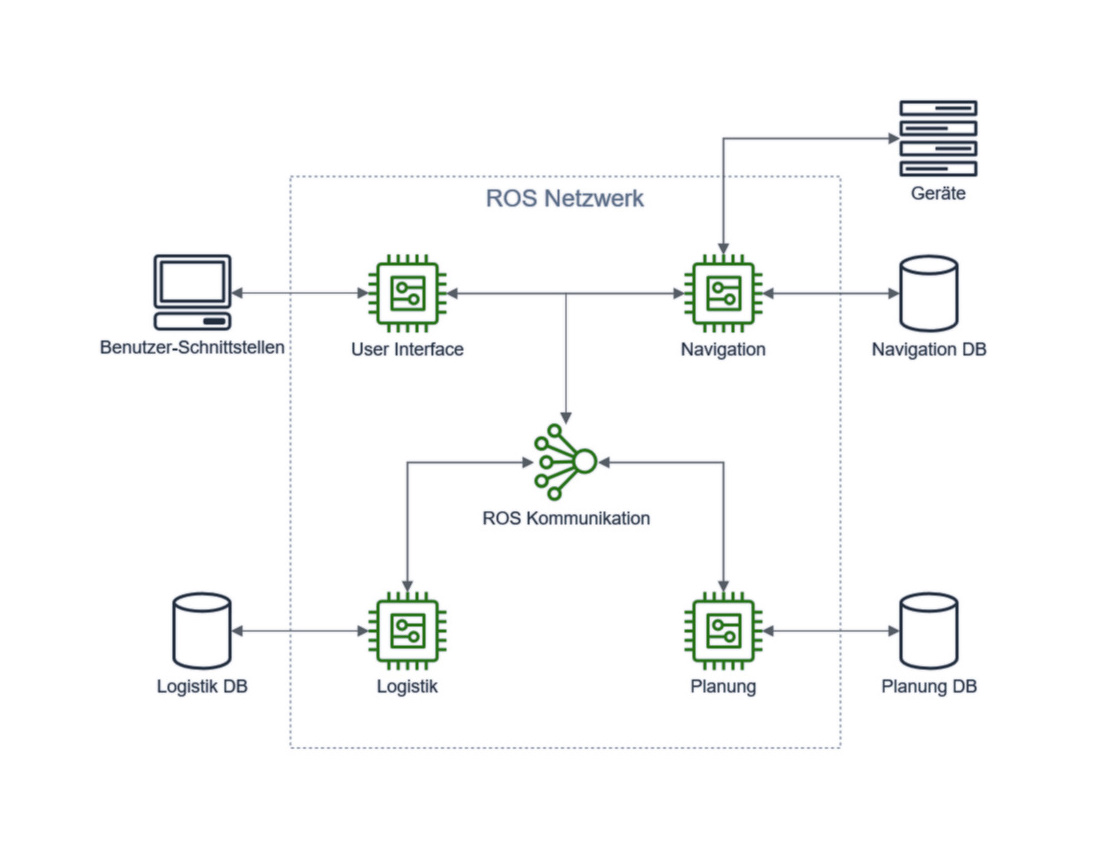
\includegraphics[width=\textwidth]{Bilder/3_ROS_Netzwerk.jpg}
\caption{Systemarchitektur}
\end{figure}

Das System ist im Kern um vier Knoten herum aufgebaut: User Interface, Logistik, Planung und Navigation. Diese vier Knoten kommunizieren untereinander, um die verschiedenen Aufgaben des Systems gemeinsam lösen zu können. Dazu umfassen der Planungs-, Navigations- und der Logistik-Knoten jeweils Datenbanken, um Pläne und Szenarien beziehungsweise Geräte und Navigationskarten sowie die verschiedenen Vorräte im Lager zu verwalten. Der Navigationsknoten unterstützt dazu die Steuerung der einzelnen Geräte, während der User Interface-Knoten die Kommunikation mit Nutzern ausführt.

Die Kommunikation zwischen den Knoten wird in den Beschreibungen der einzelnen Knoten näher erläutert. Vor allem sollte hier eine Kommunikationsart verwendet werden, die es ermöglicht, Anfragen und Befehle zwischen Knoten im System zu senden. Die Arten von Befehlen, die zur Ausführung nötig sind, werden in den Beschreibungen der einzelnen Knoten in Tabellen exemplarisch dargestellt. Dabei werden sowohl die Nachricht als auch die erwarteten Antwortmöglichkeiten als symbolischer Satz erläutert, ohne sich auf ein bestimmtes Nachrichtenformat festzulegen.

Die Kommunikation mit den Nutzern soll unabhängig über die verwendete Plattform stattfinden. Dies wird über eine generische Schnittstelle im User Interface-Knoten realisiert, die über eine Netzwerkverbindung auch ermöglicht, von externen Geräten auf das System zuzugreifen. So ist für die nachträgliche Erweiterung um neue Nutzerschnittstellen keine Änderung am System selbst nötig. Für den Entwurf dieser Benutzeroberflächen ist eine eigene UX-Konzeptionierung nötig, um die Anforderungen an eine zugängliche Semantik zu erfüllen. Da davon ausgegangen werden kann, dass die Form der Benutzeroberfläche keinen Einfluss auf die innere Funktionsweise des Systems hat, wird diese jedoch hier als gegeben angenommen.

Die Kommunikation mit den verbundenen Geräten muss ebenfalls über eine Netzwerkverbindung realisiert werden, da gerade mobile Roboter zwangsläufig nicht Teil derselben Maschine sein können. Es wird jedoch davon ausgegangen, dass sie als Teil desselben internen Netzwerks angenommen werden können, um die Kommunikation zu erleichtern und die Verbindungssicherheit zu gewährleisten. Auch wird die Steuerungsprogrammierung der eigenen Roboter als gegeben angenommen, da der Systementwurf darauf ausgelegt wird, dass die explizite Steuerung nicht durch das System durchgeführt wird. Der Entwurf der Navigationsalgorithmen ist eine eigene Forschungsaufgabe für sich, sodass hier nicht versucht wird, diese nebensächlich zu lösen.

Eine zentrale Herausforderung beim Transport von Möbeln ist, dass der Roboter in der Lage sein muss, den gewünschten Gegenstand zu identifizieren. Da größere Möbel wie Krankenliegen nicht in einem standardisierten Regal aufbewahrt werden können, muss auf eine Form der Objekterkennung zurückgegriffen werden. Es wird dafür vorausgesetzt, dass die Roboter so konzipiert sind, dass sie in der Lage sind, einen bestimmten Gegenstand zu identifizieren, wenn sie sich in der unmittelbaren Nähe befinden. Dann kann eine angepasste Version des von De La Puente et al. in \cite{assistRobot} vorgestellten Algorithmus verwendet werden, um den Gegenstand aufzuheben. Für das hier vorgestellte System wäre es dabei unerheblich, ob die Ausführung des Objekterkennungsalgorithmus auf den Robotern selbst oder einem externen Server durchgeführt wird.

Die Ausführung der Aufgabe kann dann über die von Yang et al. \cite{2DPlan} vorgestellte Methode erfolgen. Dabei wird ein Pfad von der derzeitigen Roboter-Position zu der Endposition der Aufgabe über die derzeitige Position des zu transportierenden Gegenstands geplant. Dies kann in der Regel auf einzelnen Robotern ausgeführt werden, sodass das System diese Rechenleistung nicht zur Verfügung stellen muss. Dies hat den Vorteil, dass es auf den jeweiligen Robotern vorgenommen werden kann und nur eine geringe Kommunikation mit dem zentralen Server benötigt.

Es wird sich bei der Navigation der Roboter in Situationen, in denen sie als Schwarm agieren müssen, an den Arbeiten von Reily et al. \cite{silentSwarm} orientiert. Da alle Roboter in demselben Netzwerk liegen, können sie sich gegenseitig erkennen und miteinander kommunizieren. Durch das Abrufen von Zielpunkten und Navigationskarten vom Navigationsknoten können einzelne Roboter die Wege anderer Roboter voraussagen und sich so gegenseitig ausweichen. Die Voraussetzung, dass jeder Roboter in der Lage ist, mehrere Wegplanungen gleichzeitig auszuführen, muss dafür als gegeben angenommen werden. Die Rechenlast der Wegplanung auf den einzelnen Robotern kann dadurch verringert werden, dass die Roboter auf die im Navigationsknoten liegende Karte zurückgreifen können, anstatt selbst eine erstellen zu müssen.



\FloatBarrier
\subsection{Datenbanken}

Die Datenbank des Logistik-Knotens verwaltet alle Vorräte, die vom System verwendet werden. Für das System sollte es dabei unerheblich sein, welchen individuellen Gegenstand eines Vorrats es verwendet, weshalb dieses für jeden Gegenstand eine Art festhält, nach der gesucht werden kann. Über diese Gegendstandsart kann auch, wenn erforderlich, eine genaue Spezifizierung bei zum Beispiel gesonderten Nutzungsrechten erfolgen.

Da es für den Transport durch Roboterplattformen nicht ausreicht, nur die Existenz von Gegenständen festzuhalten, muss neben der Art auch die Position im Skills Lab oder Lager festgehalten werden. Dabei sollte es auch ermöglicht werden, dass eine Art von Gegenständen über mehrere Positionen verteilt gelagert werden kann. Daher verfügt jeder individuelle Gegenstand, auch wenn dieser ansonsten identisch mit anderen in der Datenbank ist, über eine eigene Position, welche als Koordinatenpunkt festgehalten wird. Diese sind der Karte, welche dem Navigationsknoten vorliegt, zugeordnet.

Dazu ist es für die zeitkritische Planung wichtig, dass die Verfügbarkeit nicht nur zum jeweiligen Zeitpunkt festgehalten wird, sondern auch für mehrere Zeitpunkte in der Zukunft. Dementsprechend kann die Verfügbarkeit nicht nur ein Attribut eines Gegenstands sein, sondern muss auch selbstständig festgehalten werden. Deshalb muss die Datenbank in zwei verschiedene Tabellen, eine für die Suche nach Gegenständen und eine für die Suche nach Verfügbarkeiten, unterteilt werden. Dadurch kann der Logistik-Knoten ohne komplexe Algorithmen oder doppelte Einträge von Gegenständen Anfragen beantworten.

Die Datenbank des Planungsknotens ist ähnlich aufgebaut, wird aber in drei getrennten Tabellen implementiert. Die erste Tabelle fasst Szenarien mit einer für Menschen verständlichen Beschreibung sowie einen Satz für Geräte verständlicher Anweisungen. Dadurch kann sie genutzt werden, um Nutzern vorgefertigte Szenarien zur Auswahl anzubieten sowie als Grundlage der Robotersteuerung zu dienen. Dazu muss auch die Art von Gegenständen, die für jedes Szenario benötigt wird, sowie die Art des Raums, in denen dieses Szenario durchgeführt werden kann, festgehalten werden. Szenarien werden jedoch nicht für sich selbst ausgeführt, sondern fassen in erster Linie nur Befehle in einem Datenpaket zusammen, um die Planung zu erleichtern.

Um diese umzusetzen, werden geplante Szenarien in einer zweiten Tabelle eingetragen, welche die konkreten Pläne mit den dafür benötigten Geräten, spezifischen Gegenständen sowie den dafür vorgesehenen Raum umfasst. In dieser wird Szenarien zudem eine Zeitspanne zugeordnet, zu welchen diese umgesetzt werden. Sie fungiert so auch als Warteschlange, welche der Planungsknoten zu den jeweiligen Zeitpunkten in Befehle für die Navigation umwandeln kann.

Da davon ausgegangen werden kann, dass es in einem Skills Lab mehrere identisch aufgebaute Simulationsräume geben kann, werden die verfügbaren Räume in einer dritten Tabelle gespeichert, welche neben der Raumnummer auch die Art des Raums, wie sie in den Szenarien eingetragen ist, umfasst. Dadurch kann ein Plan spezifizieren, in welchem Raum er umgesetzt wird, auch wenn das Szenario auf andere, identisch aufgebaute Räume angewendet werden kann.

Die Datenbank des Navigationsknotens speichert die angeschlossenen Geräte, deren Verfügbarkeit sowie Einsatzmöglichkeiten. Der genaue Status der Geräte wird hier nicht gespeichert, da er flüchtig ist und sich insbesondere bei mobilen Robotern kontinuierlich ändern kann. Daher ist diese Datenbank ähnlich der Datenbank des Logistik-Knotens aufgebaut, die Verfügbarkeit wird genauso über eine zweite Tabelle in der Datenbank festgehalten. Statt einer Gegenstandsart wird hier jedoch über eine Liste von Schlüsselwörtern festgehalten, welche Funktion ein Gerät erfüllen kann. Dies ist vor allem für Roboter vonnöten, welche nur bestimmte Gegenstände transportieren können.



\FloatBarrier
\subsection{User Interface}

\begin{figure}[h]
\centering
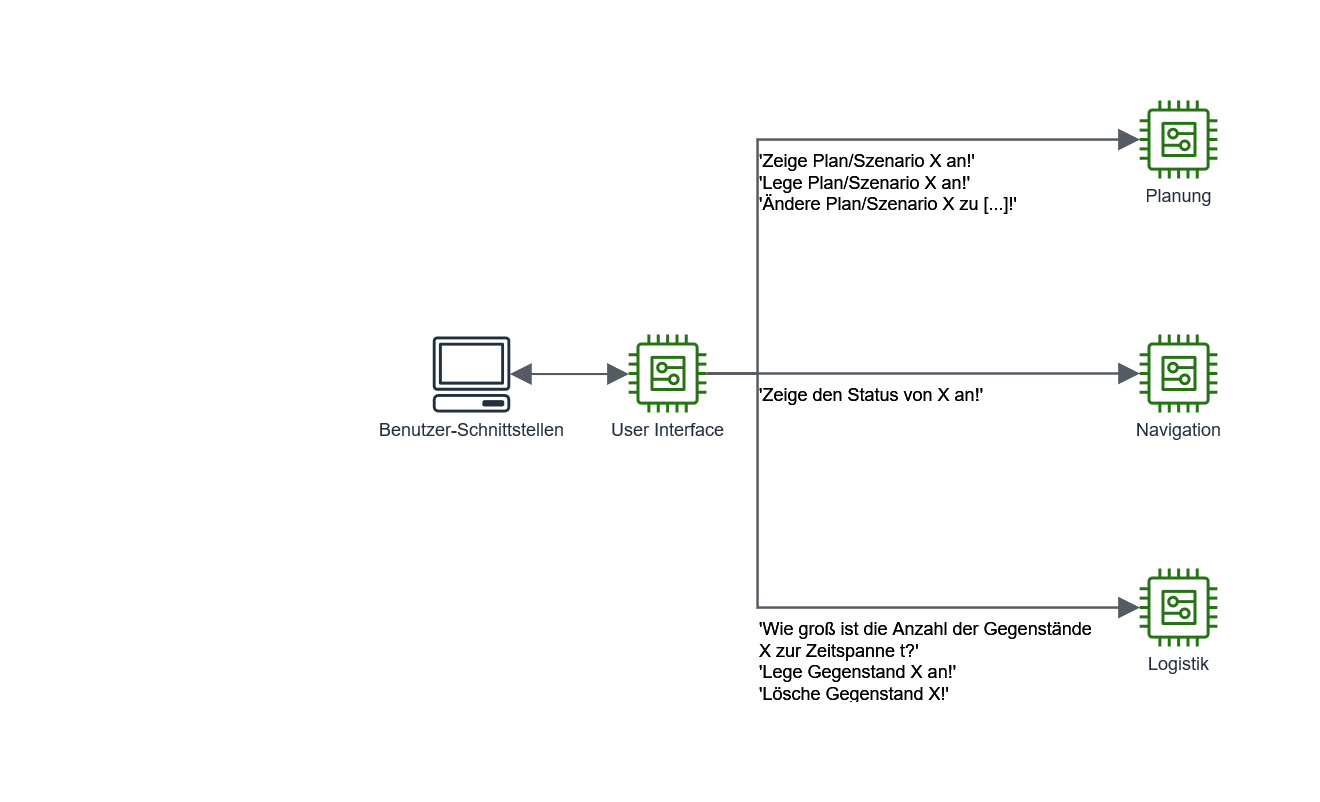
\includegraphics[width=\textwidth]{Bilder/3_User_Interface.png}
\caption{User Interface-Knoten}
\end{figure}

Der User Interface-Knoten stellt den Teil des Systems dar, mit dem Nutzer interagieren können. Er verwaltet die Kommunikation zu Nutzerschnittstellen, kann auf Anfrage Daten der Logistik, Planung und Navigation anzeigen und bündelt den Informationsfluss nach außen. Der Knoten ist auch für die Anzeige und Protokollierung von Fehlermeldungen verantwortlich. Für die Aufnahme dieser ist er in der Lage, einen gemeinsamen Kanal abzurufen und Nachrichten an diesen anzuzeigen.

Die Eingabe von auszuführenden Anweisungen an das System soll nur über den Planungsknoten erfolgen, um zu verhindern, dass Nutzerbefehle die Ausführung laufender Pläne und Szenarien stören, und zu ermöglichen, dass das System vorher überprüfen kann, ob Kollisionen mit diesen vorliegen. Daher übersetzt der User Interface-Knoten diese Nutzerbefehle nur in Systemanweisungen und leitet sie an den Planungsknoten weiter.

Hierfür werden zwei verschiedene Arten von Anweisungen verwendet. Die erste soll dazu genutzt werden, ein neues Szenario zu erstellen oder ein bestehendes anzupassen. Diese können gut zusammengefasst werden, da Szenarien nur der Vorbereitung von Handlungen dienen, aber keine Reservierungen von Geräten und Gegenständen benötigen. Die zweite Art von Anweisung soll einen neuen Plan anlegen oder einen bestehenden verändern. Damit soll es auch möglich sein, aktuell laufende Aktionen der Roboter abzubrechen oder Pläne zu löschen, da dies gut als 'einen Plan ändern' umgesetzt werden kann. Diese beiden Anweisungen werden getrennt betrachtet, da letztere eine Prüfung der verfügbaren Ressourcen und einen deutlich höheren Aufwand des Systems erfordern. In beiden Fällen soll der Nutzer aber eine Rückmeldung vom System über die vorgenommene Handlung erhalten.

Es kann unter Umständen nötig sein, dem System mitzuteilen, dass einzelne Gegenstände manuell hinzugefügt oder entfernt wurden. Dabei kann nach demselben Schema wie bei der Bearbeitung von Szenarien vorgegangen werden, da entweder eine neue Art von Gegenstand der Logistik hinzugefügt wird oder der Eintrag eines bestimmten Gegenstands verändert wird.

Um einzelne Geräte, Gegenstände, Pläne oder Szenarien anzuzeigen, kann zwischen dem User Interface-Knoten und den entsprechenden Knoten eine direkte Kommunikation stattfinden. Da hier davon ausgegangen wird, dass Nutzer keine kontinuierlichen Daten anfragen werden, kann auch hier eine Anweisung verwendet werden, die die verbundenen Knoten zu einer Anfrage auf die Datenbank veranlasst und die angeforderten Daten als Antwort zurückgibt.



\FloatBarrier
\newpage \subsection{Planung}

\begin{figure}[h]
\centering
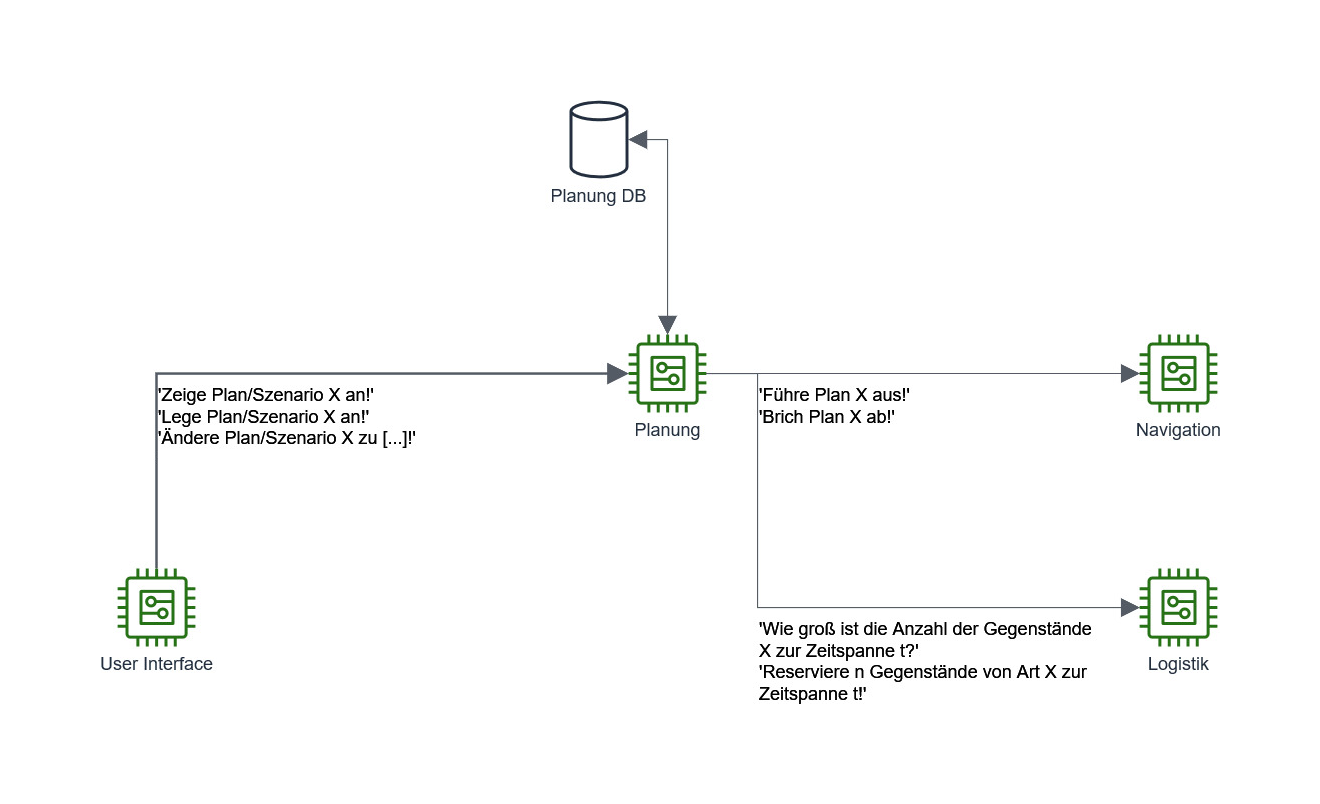
\includegraphics[width=\textwidth]{Bilder/3_Planung.png}
\caption{Planungsknoten}
\end{figure}

Die Hauptaufgaben dieses Knotens sind, Systemanweisungen von Nutzern in einzelne Befehle umzuwandeln und die erstellten Szenarien zu verwalten. Dazu muss es sowohl mit dem Logistik- als auch dem Navigationsknoten und den dazugehörigen Datenbanken kommunizieren können. Die Datenbank des Planungsknotens beinhaltet die Details der angelegten Szenarien und die zu einer bestimmten Zeit auszuführenden Pläne, wie oben beschrieben. Da davon ausgegangen wird, dass sich die Räume eines Skills Labs nicht ändern, müssen Nutzer nur direkt auf Pläne und Szenarien zugreifen können. Für das Anlegen oder Ändern von Plänen müssen zunächst die konkreten Verfügbarkeiten von Gegenständen und Geräten erfragt werden, was der Planungsknoten automatisch für den Nutzer ausführt. Basierend auf den Verfügbarkeiten gibt er dem Nutzer Feedback, ob ein Plan umsetzbar ist und trägt diesen gegebenenfalls auch in die Warteschlange der Pläne ein.

Damit Pläne umgesetzt werden, muss der Knoten selbstständig überprüfen, welcher als nächstes auszuführen ist, um zu dem angegebenen Zeitpunkt die entsprechenden Anweisungen an den Navigationsknoten geben zu können. Der Planungsknoten stellt dadurch das zentrale Element bei der Ausführung von vorher festgelegten Szenarien dar. Der Navigationsknoten gibt den Status der momentan ausgeführten Pläne dabei an den Planungsknoten zurück. Dadurch kann der Planungsknoten die an die Navigation gegebenen Anweisungen überwachen und gegebenenfalls die Planung anpassen. Falls ein Plan während der Ausführung geändert wird, wird der Navigationsknoten informiert, dass die jeweilige Aktion abgebrochen wird. Danach sendet der Planungsknoten einen neuen Plan, um die Änderungen umzusetzen. Auch hier wird eine Rückmeldung des Navigationsknotens erwartet, bis eine Bestätigung erfolgt, dass die Aktion vollständig abgebrochen wurde.

Ein Nutzer kann über das User Interface auf den Planungsknoten zugreifen, um neue Pläne und Szenarien anzulegen, bestehende anzuzeigen oder zu ändern. Der Knoten prüft bei neu angelegten oder geänderten Einträgen, ob dieser ausgeführt werden kann, indem entsprechende Anweisungen an die Logistik- und Planungsknoten gesandt werden. Falls dies der Fall ist, übersetzt der Knoten die ursprüngliche Anweisung in eine Datenbankanfrage und gibt zuletzt das Ergebnis als Rückmeldung zurück.

\begin{table}[h]
\begin{center}
\begin{tabular}{| r l |}
  \hline
  Anweisung  & \dq Zeige Plan/Szenario X an!\dq  \\
  \hline
  Rückmeldung & \dq Plan/Szenario X umfasst [..].\dq  \\
  oder     & \textbf{\dq Plan/Szenario X ist nicht bekannt.\dq } \\
  \hline
  \hline
  Anweisung  & \dq Lege Plan/Szenario X an!\dq  \\
  \hline
  Rückmeldung & \dq Plan/Szenario X angelegt.\dq  \\
  oder     & \textbf{\dq Plan/Szenario X existiert schon.\dq } \\
  \hline
  \hline
  Anweisung  & \dq Ändere Plan/Szenario X zu [..]!\dq \\ 
  \hline
  Rückmeldung & \dq Plan/Szenario X umfasst [..].\dq  \\  
  oder     & \dq Vorrat für Plan/Szenario X nicht ausreichend.\dq \\
  oder     & \textbf{\dq Plan/Szenario X ist nicht bekannt.\dq }\\
  \hline
  \hline
\end{tabular}  
\caption{Kommunikation von User Interface zu Planung}
\end{center}
\end{table}


\FloatBarrier
\newpage \subsection{Navigation}

\begin{figure}[h]
\centering
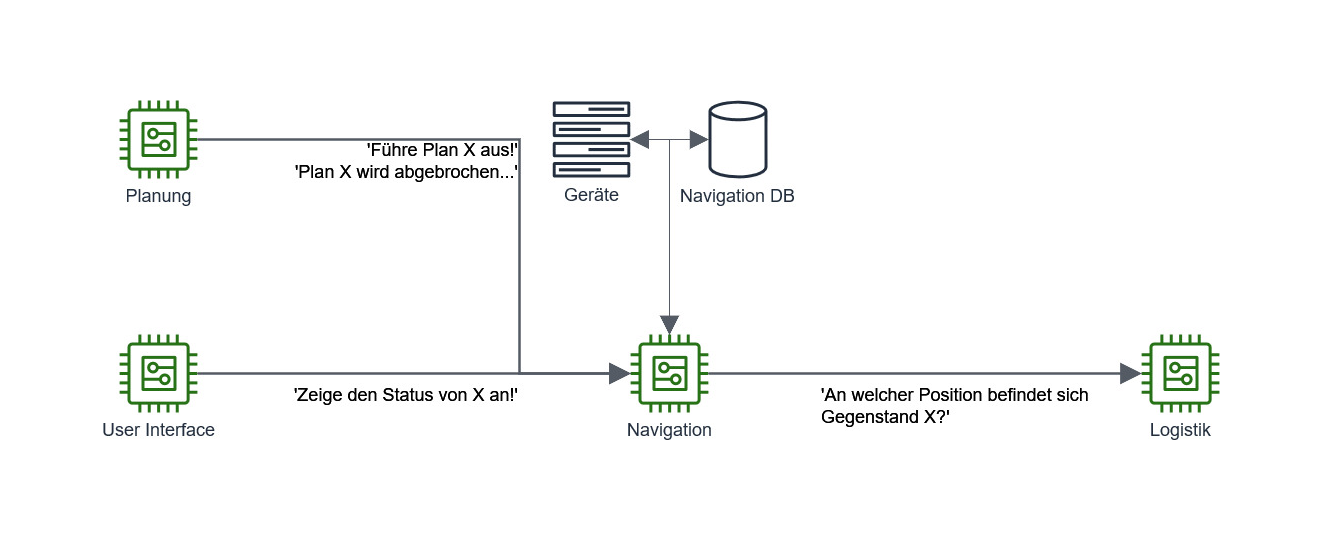
\includegraphics[width=\textwidth]{Bilder/3_Navigation.png}
\caption{Navigationsknoten}
\end{figure}

Der Navigationsknoten ist für die Steuerung der verbundenen Geräte, insbesondere der Roboter, nach den übermittelten Anweisungen des Planungsknotens verantwortlich. Er wandelt diese in für die Roboter ausführbare Navigationsanweisungen um und überwacht den Status der Geräte während der Ausführung.

Der Planungsknoten wird im laufenden Betrieb den Großteil seiner Anfragen an die Navigation senden. Dies erfolgt über zwei Arten von Anweisungen. Die erste weist die Navigation an, einen Plan auszuführen, der in der Nachricht spezifiziert wird. Ein solcher Plan beinhaltet ein Szenario, den Raum, in dem dieses umgesetzt werden soll, sowie die Gegenstände, die verwendet werden sollen. Aus diesen berechnet der Navigationsknoten die Route von geeigneten Geräten und gibt diesen die entsprechenden Befehle.

Um dies umzusetzen, muss der Knoten über eine Navigationskarte verfügen, die das gesamte Skills Lab inklusive Lager umfasst. Dazu muss eine Datenbank der ansprechbaren Geräte entsprechend der oben beschriebenen Vorlage angebunden sein. Aus dieser Datenbank kann der Planungsknoten die zu verwendenden Geräte für eine Handlung auswählen, um ihnen dann die Anweisungen zu erteilen. Hierfür muss der Navigationsknoten zuletzt auch die Position der zu transportierenden Gegenstände vom Logistik-Knoten erfragen, was über die bekannte Anweisung/Rückmeldung-Kommunikation erfolgt.

Um die Anforderung zu erfüllen, Pläne während der Ausführung ändern oder abbrechen zu können, kann der Planungsknoten zudem eine Anweisung senden, um die Ausführung eines Plans abzubrechen. Bei Eingang einer solchen Anfrage sendet der Navigationsknoten an die Geräte den Befehl, alle derzeitigen Aktionen abzubrechen und im Falle von mobilen Plattformen zu ihrer üblichen Ruheposition zurückzukehren oder eine neue Aufgabe zu übernehmen. Falls Roboter in dem Moment Gegenstände transportieren, werden sie zudem angewiesen, vorher diese zurück zu der Ausgangsposition zu bewegen. Erst, wenn alle Geräte wieder für neue Aufgaben verfügbar sind, wird die Rückmeldung gesendet, dass die Aktion abgebrochen wurde.

In beiden Fällen kann es eine gewisse Zeit dauern, bis die Rückmeldung gesendet wird. Daher sendet der Navigationsknoten in regelmäßigen Abständen Statusmeldungen an den Planungsknoten. Diese Meldungen geben diesem Rückmeldung, ob der Plan ohne Zwischenfall ausgeführt wird oder Probleme aufgetaucht sind, welche die Ausführung verzögern oder gar unmöglich machen.

\begin{table}[h]
\begin{center}
\begin{tabular}{| r l |}
  \hline
  Anweisung  & \dq Führe Plan X aus!\dq  \\
  \hline
  Rückmeldung & \dq Plan X wird ausgeführt..\dq  \\
           & Navigation fängt an, Feedback zu geben \\
  oder     & \textbf{\dq Plan X kann nicht ausgeführt werden.\dq } \\
  \hline
  \hline
  Anweisung  & \dq Brich Plan X ab!\dq  \\
  \hline
  Rückmeldung & \dq Plan X wird abgebrochen..\dq  \\
           & Navigation fängt an, Feedback zu geben \\
  oder     & \textbf{\dq Plan X kann nicht abgebrochen werden.\dq } \\
  oder     & \textbf{\dq Plan X ist nicht bekannt.\dq } \\
  \hline
\end{tabular}  
\caption{Kommunikation von Planung zu Navigation}
\end{center}
\end{table}

Ein Nutzer kann über den User Interface-Knoten direkt eine Anweisung senden, um den Status eines Geräts zu erfragen. Um diese zu beantworten, muss der Knoten eine eigene Anfrage an das entsprechende Gerät senden. Da der Status von Geräten je nach Art Unterschiedliches umfassen kann, wird davon ausgegangen, dass der Navigationsknoten diesen für die Rückmeldung an das User Interface übersetzen muss, ehe er weitergegeben wird.

\begin{table}[h]
\begin{center}
\begin{tabular}{| r l |}
  \hline
  Anweisung  & \dq Zeige den Status von X an!\dq  \\
  \hline
  Rückmeldung & \dq Der Staus von X ist [..].\dq  \\
  oder     & \textbf{\dq Gerät X nicht bekannt.\dq } \\
  \hline
\end{tabular}  
\caption{Kommunikation von User Interface zu Navigation}
\end{center}
\end{table}


\FloatBarrier
\newpage \subsection{Logistik}

\begin{figure}[h]
\centering
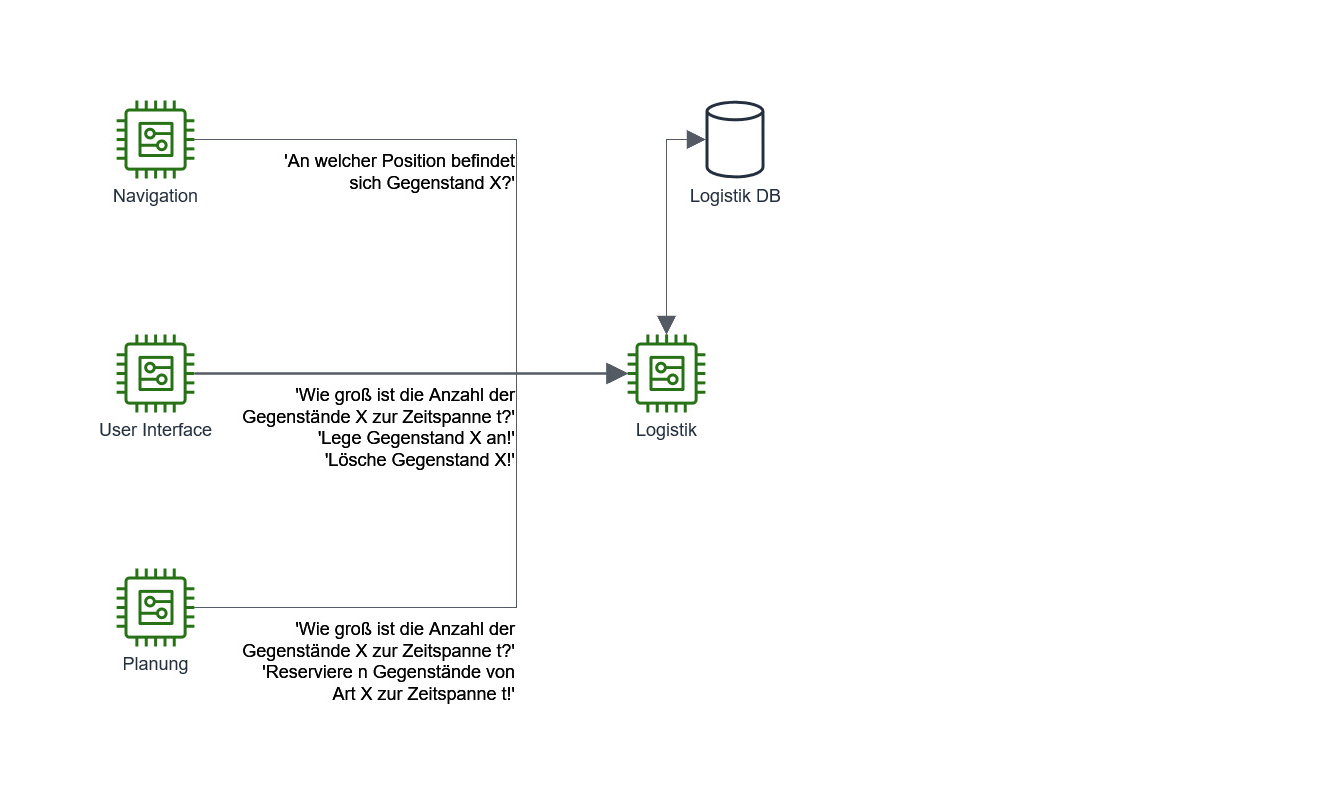
\includegraphics[width=\textwidth]{Bilder/3_Logistik.png}
\caption{Logistik-Knoten}
\end{figure}

Der Logistik-Knoten ist der Einzige, der selbstständig keine Anfragen an andere sendet. Er ist nur für die Kommunikation mit der entsprechenden Datenbank und die Aufbereitung der darin enthaltenen Informationen für andere Knoten verantwortlich. Der Logistik-Knoten kann Anweisungen von allen anderen Knoten erhalten.

Der User Interface-Knoten kann drei verschiedene Anweisungen an den Logistik-Knoten senden. Zum einen kann er erfragen, wie viele Gegenstände einer bestimmten Art zu einer bestimmten Zeitspanne verfügbar sind. Da die Datenbank für jeden Gegenstand Einträge für die blockierten Zeiten besitzt, kann der Knoten eine Datenbank-Anfrage darauf durchführen und die entsprechende Anzahl zurückgeben. Dazu können die Anweisungen kommen, einen neuen Gegenstand anzulegen oder einen bestehenden zu löschen. Beides sind ebenfalls einfache Datenbank-Anfragen, welche der Knoten in einer Rückmeldung mit den Einträgen beantworten kann.

Für die Planung ist es notwendig, dass die Anzahl der verfügbaren Gegenstände zu einer gegebenen Zeitspanne bekannt sind und eingeplante Gegenstände reserviert werden können. Bei einer Reservierung von Gegenständen sucht der Logistik-Knoten die angefragte Anzahl der gegebenen Art aus der Datenbank und fügt der Logistik-Tabelle die entsprechenden Gegenstände hinzu. Dabei müssen die Gegenstände zu dieser Zeitspanne auch verfügbar sein, sodass der Knoten bei der Auswahl die bestehenden Reservierungen mit der angefragten Spanne vergleicht.

Für die Navigation wird davon ausgegangen, dass die Planung korrekt erfolgt ist, bevor die Ausführung der Navigation überlassen wird. Dementsprechend wird von diesem Knoten nur eine Anweisung gesendet, die die derzeitige Position des gesuchten Gegenstands erfragt. Dies ist wieder eine einfache Datenbank-Anfrage, deren Antwort in der Rückmeldung zurückgegeben werden kann.

\begin{table}[h]
\begin{center}
\begin{tabular}{| r l |}
  \hline
  Anweisung  & \dq Wie groß ist die Anzahl der Gegenstände X zur Zeitspanne t?\dq  \\
  \hline
  Rückmeldung & \dq Die Anzahl der Gegenstände X zur Zeitspanne t beträgt n.\dq  \\
  oder     & \textbf{\dq Gegenstand X ist nicht bekannt.\dq } \\
  \hline
  \hline
  Anweisung  & \dq Lege Gegenstand X an!\dq  \\ 
  \hline
  Rückmeldung & \dq Gegenstand X angelegt.\dq  \\  
  oder     & \dq Vorrat X nicht ausreichend.\dq  \\
  oder     & \textbf{\dq Gegenstand X existiert schon.\dq } \\
  \hline
  \hline
  Anweisung  & \dq Lösche Gegenstand X!\dq  \\
  \hline
  Rückmeldung & \dq Gegenstand X gelöscht.\dq  \\
  oder     & \textbf{\dq Gegenstand X ist nicht bekannt.\dq } \\
  \hline
\end{tabular}  
\caption{Kommunikation von User Interface zu Logistik}
\end{center}
\end{table}

\begin{table}[h]
\begin{center}
\begin{tabular}{| r l |}
  \hline
  Anweisung  & \dq Reserviere n Gegenstände von Art X zur Zeitspanne t!\dq  \\
  \hline
  Rückmeldung & \dq Zur Zeitspanne t sind n Gegenstände der Art X reserviert.\dq  \\
  oder     & \textbf{\dq Gegenstand der Art X ist nicht bekannt.\dq } \\
  \hline
\end{tabular}  
\caption{Kommunikation von Planung zu Logistik}
\end{center}
\end{table}

\begin{table}[h]
\begin{center}
\begin{tabular}{| r l |}
  \hline
  Anweisung  & \dq An welcher Position befindet sich Gegenstand X?\dq  \\
  \hline
  Rückmeldung & \dq Gegenstand X befindet sich an Position XY.\dq  \\
  oder     & \textbf{\dq Gegenstand X ist nicht bekannt.\dq } \\
  \hline
\end{tabular}  
\caption{Kommunikation von Navigation zu Logistik}
\end{center}
\end{table}
\setcounter{section}{0}

\addtocounter{chapter}{1}
\part{Implementierung\label{Implementierung}}
\section{Verwendete Tools}

Für die Implementierung des gewünschten Systems muss ein Framework verwendet werden, in dem alle diese gegebenen Anforderungen erfüllt werden können. Dieses selbst zu implementieren würde sowohl nicht dem Rahmen einer Bachelorarbeit entsprechen als auch voraussichtlich nicht die Möglichkeiten bestehender Werkzeuge erreichen, weshalb eine vorgefertigte Lösung verwendet wird.

Das Robot Operating System 2 von Open Robotics \cite{ros}, welches dafür konzipiert wurde, eine Kommunikation zwischen Robotern und anderen Computern in nahezu Echtzeit zu ermöglichen, ist als Framework für diese Art von System geeignet. Dieses erfüllt die Anforderung an die Skalier- und Erweiterbarkeit, da es sowohl über einen zentralen als auch verteilte Knoten betrieben werden kann und daher mit dem System wächst, ohne einen Engpass darzustellen. Auch ist es ein Open Source-Framework und verfügt über eine öffentlich zugängliche Dokumentation, sodass in dieser Hinsicht die Erweiterung durch Dritte keinerlei Probleme darstellen sollte. Es kann unter Windows, Ubuntu Linux, macOS und RHEL installiert und betrieben werden und unterstützt nativ die Programmierung von Knoten in den Sprachen Python und C++.

Ein Netzwerk in ROS ist um eine Mehrzahl von Knoten herum aufgebaut. Diese können einzelne Roboter, Geräte oder Prozesse innerhalb des System-Netzwerks darstellen. ROS ermöglicht es, zwischen Knoten verschiedene Dateninhalte über sogenannte Topics, Services und Actions zu teilen. Topics stellen dabei eine Ein-Wege-Kommunikation auf einem ständig offenen Kanal dar. Knoten können an Topics Nachrichten senden und von diesen solche empfangen, wobei es unerheblich ist, wie viele Knoten Nachrichten von einem Topic lesen. Dadurch können in Echtzeit Statusmeldungen und sich kontinuierlich ändernde Daten geteilt werden.

Services dagegen stellen eine Zwei-Wege-Kommunikation dar, bei der ein Client-Knoten einen bestimmten Service von einem Server-Knoten anfragt. Knoten, welche als solche Service Server konfiguriert wurden, senden Nachrichten nur dann, wenn über einen Request des Service Clients diese angefordert werden. Dies verhindert, dass selten benötigte oder sich nur selten ändernde Daten unnötige Bandbreite belegen, indem sie kontinuierlich gesendet werden müssen. Auch können so Anweisungen von einem Knoten an einen anderen gegeben werden.

Actions sind eine erweiterte Form von Services, bei denen davon ausgegangen wird, dass die Beantwortung einer Anfrage eine gewisse Zeit in Anspruch nimmt. Nach einer Bestätigung einer Anfrage sendet daher der Server-Knoten auf einem Topic Statusmeldungen, um den Client-Knoten über den Fortschritt der Anweisung zu informieren, bis die Anfrage abschließend bearbeitet wurde. Dies wird vor allem dann benutzt, wenn cyber-physikalische Systeme angesprochen werden, die andauernde Aktionen ausführen. 

Durch diese Kommunikationswege ist es für das System möglich, sowohl für die Kommunikation zu Geräten als auch zu Schnittstellen der Benutzeroberfläche dieselbe Middleware zu verwenden und den Nachrichtenversand an die Anforderungen anzupassen. Dadurch kann auch nativ ein Multi-User Konzept für die Eingabe von Nutzeranweisungen realisiert werden, in welchem jeder Zugang einen eigenen Knoten darstellt, welcher über entsprechende Topics mit dem System kommuniziert. Alle Nachrichten können in ROS standardmäßig auf der Kommunikationsebene verschlüsselt und authentifiziert werden, sodass der Nutzerzugang über gesicherte Schnittstellen sicher gestellt werden kann.

Zur Programmierung der Knoten wird in diesem Projekt die Programmiersprache Python verwendet. Eine Verwendung von C++ oder anderer Sprachen, welche durch Einbindung von Drittpartei-Libraries unterstützt werden könnten, könnte unter Umständen die Ausführung des Systems beschleunigen. Da diese jedoch im Vergleich zu Netzwerk-Latenzen und Datenbank-Zugriffsgeschwindigkeiten vernachlässigbar klein sind, stellt Python als weit verbreitete und leicht zu erlernende Sprache durch die Erleichterung der Erweiterbarkeit durch Dritte die bessere Wahl dar.

Die Datenbanken werden in der Implementierung mithilfe von SQLite3 erstellt, einer Library zu Erstellung von ressourcenschonenden Datenbanken. Es basiert auf der SQL-Sprache, welche die Basis für die meisten Datenbanksysteme ist. SQLite bietet die Möglichkeit, Befehle direkt in Python-Programmen zu verwenden, sodass keine externe Software zur Übersetzung nötig ist.


\FloatBarrier
\section{Systemarchitektur}

Die Umsetzung der Systemarchitektur wird mithilfe voneinander unabhängiger ROS-Knoten umgesetzt, welche in einer gemeinsamen Umgebung kompiliert werden, allerdings auch als einzelne Pakete ausgeführt werden können. Jeder Knoten besteht dabei aus einem Kern-Knoten, welcher zuerst initialisiert wird und den Ansprechpartner für andere Knoten darstellt. Dazu verfügen die einzelnen Kern-Knoten zum Teil über sekundäre Knoten, auf die bestimmte Aufgaben ausgelagert werden, um eine Parallelisierung von Abläufen zu ermöglichen. Diese werden in den einzelnen Knoten-Beschreibungen näher erläutert.

Die Implementierung unterscheidet sich in zwei Punkten von dem Gesamtkonzept und erfüllt bisher nicht alle Ansprüche des Systems, um der Arbeit einen angemessenen Umfang zu geben. Zum einen wird dadurch, dass von einer später zu entwickelnden Nutzerschnittstelle ausgegangen wird, stattdessen eine Befehlseingabe per Konsole zur Verfügung gestellt. Diese ermöglicht, alle implementierten Funktionen des Systems direkt zu nutzen, ohne eine dedizierte Plattform bereitstellen zu müssen. Dazu sind einige Nutzereingaben, die über das Ziel der Implementierung hinausgehen, implementiert worden, um die Entwicklung und das Testen des Systems zu vereinfachen.

Da die explizite Implementierung von Navigationsstrategien von Robotern nicht Ziel dieser Arbeit ist, verfügt die hier vorgestellte Lösung zum anderen auch über keinen Navigationsknoten oder dazugehörige Services. Insbesondere stehen keine verwendbaren Navigationsbefehle in der Datenbank des Planungsknotens zur Verfügung. Auch ist auf eine Umsetzung der Warteschlange für auszuführende Pläne verzichtet worden, da durch den nicht implementierten Navigationsknoten die Abfrage von diesen nicht erfolgt.

Die Kommunikation zwischen den Knoten wird über sogenannte Interfaces definiert, welche einen Rahmen für die jeweiligen Nachrichten bieten. In dieser Implementierung werden nur eigene Interfaces für Services verwendet, welche dementsprechend die Dateiendung '.srv' besitzen. Jedes dieser Interfaces kann eine Mehrzahl an Argumenten unter einem Alias und einer Spezifikation des verwendeten Datentyps für jeweils den Service-Aufruf und die Antwort aufnehmen.

Diese Interfaces sind hier nach dem jeweiligen Verwendungszweck zusammengefasst. Services, welche sich mit Gegenständen befassen, verwenden das Interface 'Item.srv', solche für Szenarien 'Goal.srv', jene für Pläne 'Plan.srv' und diejenigen, die sich mit dem Anlegen von Datenbanken befassen, 'MakeDB.srv'. Die jeweiligen Argumente der Interfaces samt Datentyp und Verwendungszweck sind in der folgenden Tabelle aufgeführt.

\begin{table}[h]
\begin{center}
\begin{tabular}{| c | c | c | l |}
  \hline
  Interface & Datentyp & Argument & Verwendungszweck \\
  \hline
  \hline
  Item.srv   & int32   & id            & ID-Nummer eines bestimmten Gegenstandes\\
             & string  & item\_kind    & Art eines Gegenstandes\\
             & string  & position      & Position eines Gegenstandes in 2D-Ebene\\
             & int32   & begin\_date   & Anfangszeit einer Reservierung\\
             & int32   & end\_date     & Abschlusszeit einer Reservierung\\
             & bool    & ack           & Antwort - Bestätigung eines Aufgabeneingangs\\
             & int32[] & reserved\_ids & Antwort - ID-Nummern reservierter Gegenstände\\
  \hline
  \hline
  Goal.srv   & int32   & goal\_id      & ID-Nummer eines bestimmten Szenarios\\
             & string  & goal\_desc    & Beschreibung eines Szenarios\\
             & string  & goal\_nav     & Navigationsbefehle des Szenarios\\
             & bool    & ack           & Antwort - Bestätigung eines Aufgabeneingangs\\
  \hline
  \hline
  Plan.srv   & int32   & id            & ID-Nummer eines bestimmten Plans\\
             & int32   & goal\_id      & ID-Nummer des angewendeten Szenarios\\
             & string  & items         & Liste der verwendeten Gegenstände\\
             & int32   & begin\_time   & Anfangszeit eines Plans\\
             & int32   & end\_time     & Abschlusszeit eines Plans\\
             & bool    & ack           & Antwort - Bestätigung eines Aufgabeneingangs\\
  \hline
  \hline
  MakeDB.srv & string  & db\_name      & Name der anzulegenden Datenbank\\
             & bool    & ack           & Antwort - Bestätigung eines Aufgabeneingangs\\
  \hline
  \hline
  String.msg & string  & user\_info    & Senden der Systemmitteilungen an Nutzer\\
  \hline
\end{tabular}
\caption{Verwendete Interfaces}
\end{center}
\end{table}

Das Topic 'user\_information', an welches Knoten für Nutzer relevante Informationen über ihre ausgeführten Aufgaben teilen, benötigt kein eigenes Interface. Hier kann das in ROS2 vorhandene String-Format verwendet werden, da in dieser Implementierung nur Textzeilen übertragen werden.


\FloatBarrier
\section{User Interface}

Der User Interface-Knoten ist aus drei ROS-Knoten aufgebaut: dem 'NodeUICore', den 'NodeUICommunicator' und dem 'NodeUIOutput'. Der NodeUICore nimmt Nutzereingaben entgegen und gibt diese an den NodeUICommunicator weiter. Dieser übersetzt Nutzereingaben in Service-Anfragen an andere Knoten. NodeUIOutput nimmt die auf dem Topic 'user\_interface' geteilten Nachrichten und gibt sie in einem eigenen Konsolen-Fenster aus.

NodeUICore initialisiert beim Start auch NodeUICommunicator, um an die Planungs- und Logistikknoten die Anweisung zu übermitteln, sich mit den jeweiligen Datenbanken zu verbinden. Ansonsten verfügt die Klasse nur über ein Attribut 'service\_choice', welches die Eingabe zur Weitergabe beinhaltet. Nach der Initialisierung ruft der Knoten die Funktion 'select\_service()' auf, mittels der dem Nutzer die wählbaren Optionen angezeigt werden und eine Auswahl per Konsoleneingabe angenommen wird. Diese Auswahl wird über das Attribut service\_choice dann an NodeUICommunicator per Funktionsaufruf weitergegeben. Die Ausführung von select\_service() kann über einen Befehl 'close\_ui' unterbrochen werden, wodurch der Knoten anschließend terminiert.

\begin{table}[h]
\begin{center}
\begin{tabular}{| c | l | c |}
  \hline
  Nutzereingabe & Aktion & Ausführender Knoten\\
  \hline
  \hline
  show\_item    & zeigt einen Gegenstand an           & Logistik \\
  show\_goal    & zeigt ein Szenario an               & Planung  \\
  show\_plan    & zeigt einen Plan an                 & Planung  \\
  create\_item  & erstellt einen neuen Gegenstand     & Logistik \\
  create\_goal  & erstellt ein neues Szenario         & Planung  \\
  create\_plan  & erstellt einen neuen Plan           & Planung  \\
  edit\_item    & ändert die Daten eines Gegenstandes & Logistik \\
  edit\_goal    & ändert die Daten eines Szenarios    & Planung  \\
  edit\_plan    & ändert die Daten eines Plans        & Planung  \\
  delete\_item  & löscht einen Gegenstand             & Logistik \\
  delete\_goal  & löscht ein Szenario                 & Planung  \\
  delete\_plan  & löscht einen Plan                   & Planung  \\
  close\_ui     & schließt den User Interface-Knoten  & ---      \\
  \hline
\end{tabular}
\caption{Verfügbare Befehle}
\end{center}
\end{table}

Bei der Initialisierung von NodeUICommunicator werden im Gegensatz zum Kern-Knoten keinerlei Handlungen ausgeführt. Der Knoten wird stattdessen nur zur Ausführung einzelner Funktionsaufrufe verwendet, nach denen der Knoten wieder geschlossen wird. Der Aufruf findet über die oben beschriebene Funktion select\_service von NodeUICore statt. Jede der Funktionen fügt die gegebenenfalls erforderlichen Konsoleneingaben zu einer Service Request zusammen, um diese Request dann an den Knoten zu senden, der in der Tabelle 'Verfügbare Befehle' angegeben ist.

\begin{figure}
\begin{center}
\begin{tikzpicture}
\begin{umlpackage}{User Interface}
\umlclass{NodeUICore}
{service\_choice : string \\
 node\_comm : Node = NodeUICommunicator()}
{select\_service() : void}

\umlclass[x=8, y=-5]{NodeUICommunicator}
{input : string}
{make\_plan\_db() : MakeDB.Request()\\
 show\_item(input) : Item.Request()\\
 show\_goal(input) : Goal.Request()\\
 show\_plan(input) : Plan.Request()\\
 create\_item(input) : Item.Request()\\
 create\_goal(input) : Goal.Request()\\
 create\_plan(input) : Plan.Request()\\
 edit\_item(input) : Item.Request()\\
 edit\_goal(input) : Goal.Request()\\
 edit\_plan(input) : Plan.Request()\\
 delete\_item(input) : Item.Request()\\
 delete\_goal(input) : Goal.Request()\\
 delete\_plan(input) : Plan.Request()\\
 close\_ui() : void
}

\umlclass[x=0, y=-5]{NodeUIOutput}
{subscription : create\_subscription() \\
 msg : string}
{listener\_callback(msg) : void}

\umluniassoc[geometry = -|, arg1=select\_service(), align1=left]
{NodeUICore}{NodeUICommunicator}
\end{umlpackage}
\end{tikzpicture}
\caption{User Interface-Knoten: Klassendiagramm}
\end{center}
\end{figure}

Zuletzt liegt der Knoten NodeUIOutput im Paket, welcher keine Interaktion mit den anderen beiden Knoten ausführt. Die einzige Aufgabe des Knotens ist, Nachrichten an das Topic 'user\_information' zu empfangen und auf einer Konsole auszugeben. Dementsprechend verfügt der Knoten auch nur über die Funktion 'listener\_callback(msg)', welche die empfangenen Nachrichten mit einem Zeitstempel druckt.


\FloatBarrier
\section{Planung}

Das Paket des Planungsknotens ist ähnlich dem vorangehenden User Interface aufgebaut, auch hier gibt es einen Kern- und einen Kommunikationsknoten, 'NodePlanCore' und 'NodePlanCommunicator' genannt. NodePlanCore nimmt hier aber Service Requests anderer Knoten entgegen, um diese zu bearbeiten. Hierfür besteht auch eine Verbindung zu der Datenbank des Planungsknotens, um SQL-Befehle an diese zu geben.

NodePlanCore dient als Service Server für eine Vielzahl von Funktionen, deren Verbindungsschnittstellen bei der Initialisierung geöffnet werden. All diese Services rufen eine eigene Rückruffunktion mit dem Namen 'callback\_(Name des Service)' auf, welche der Request mit den übermittelten Parametern entgegennehmen und nach Abschluss auf diese antworten. Zur Umsetzung des Services wird dann eine Datenbank-Funktion mit dem Namen 'db\_(Name des Service)' aufgerufen, welche die Parameter der Request erhält und die entsprechende Aktion ausführt. Nach Abschluss der Datenbank-Funktion sendet die Rückruffunktion dann eine Bestätigung des Services zurück und sendet zusätzlich eine Nachricht an das Topic 'user\_information', in der die gerade vorgenommene Aktion beschrieben ist.

\begin{table}[h]
\begin{center}
\begin{tabular}{| c | c | l |}
  \hline
  Service        & Interface & Parameter                                         \\
  \hline
  \hline
  make\_plan\_db & MakeDB    & ---                                               \\
  show\_goal     & Goal      & goal\_id                                          \\
  show\_plan     & Plan      & plan\_id                                          \\
  create\_goal   & Goal      & goal\_desc                                        \\
  create\_plan   & Plan      & goal\_id, items, begin\_time, end\_time           \\
  edit\_goal     & Goal      & goal\_desc, goal\_id                              \\
  edit\_plan     & Plan      & plan\_id, goal\_id, items, begin\_time, end\_time \\
  delete\_goal   & Goal      & goal\_id                                          \\
  delete\_plan   & Plan      & plan\_id                                          \\
  \hline
\end{tabular}
\caption{Planungsknoten: Ausführbare Services}
\end{center}
\end{table}

Die Datenbank-Funktionen der jeweiligen Services fügen aus den weitergegebenen Parametern der Request und einem generischen SQL-Befehl die Anweisung an die Datenbank zusammen und lassen diese ausführen. Daten der verwendeten Tabelle, die von der Rückruffunktion erwartet werden, werden in dieser von der Datenbank-Funktion ausgelesen. Dieses Schema trifft einzig nicht auf die Funktion 'callback\_create\_plan' zu, da diese zusätzlich zu dem Datenbank-Aufruf auch einen Service Request an den Logistik-Knoten senden muss, um die benötigten Gegenstände zu reservieren. Hierzu wird bei Funktionsaufruf erst eine Anfrage an den Logistik-Knoten mit den benötigen Gegenstandsarten gesendet, um festzustellen, ob der anzulegende Plan umsetzbar ist. Im Falle einer positiven Response wird dann die ursprüngliche Request, welche um die ID-Nummern der reservierten Gegenstände erweitert wurde, an die Datenbank-Funktion weitergegeben.

\begin{figure}
\begin{center}
\begin{tikzpicture}
\begin{umlpackage}{Planung}
\umlclass{NodePlanCore}
{conn : sqlite3.connect(self.db\_file) \\
 msg : string \\
 node\_comm : Node = NodePlanCommunicator()\\
 srv\_$*$ : create\_service()
 publisher\_ : create\_publisher()}
{callback\_$*$(request, response) : response \\
 db\_$*$(request) : Datenbank-Antwort}

\umlclass[x=0, y=-5]{NodePlanCommunicator}
{}
{reserve\_item(item\_kind, begin\_date, end\_date) : Item.Request()}

\umluniassoc[arg1=create\_plan()]
{NodePlanCore}{NodePlanCommunicator}
\end{umlpackage}
\end{tikzpicture}
\caption{Planungsknoten: Klassendiagramm}
\end{center}
\end{figure}

Die Datenbank selbst ist in drei Tabellen unterteilt: 'goals', 'rooms' und 'goal\_planning'. Die erste Tabelle nimmt die einzelnen Szenarien, in der Implementierung ebenfalls als 'goals' bezeichnet, auf und speichert neben der jeweiligen ID-Nummer auch die Beschreibung des Szenarios und die benötigten Gegenstände und Räume. Dazu soll die Tabelle auch die Navigationsanweisungen enthalten, mit denen der Plan ausgeführt werden kann. Da diese aber noch nicht erstellt sind, wird derweil ein Platzhalter verwendet.

'rooms' umfasst dagegen die verfügbaren Räume, sodass in der Planung freie Räume gesucht werden können. Die Tabelle goal\_planning verweist auf die erste und zweite Tabelle, versieht die Szenarien jedoch mit konkreten ID-Nummern für die Gegenstände und Räume und einer Zeitspanne zur Ausführung. Die Zeitspanne ist dabei in UNIX Time angegeben, da diese von nahezu allen Maschinen gelesen und verwendet werden kann. Für jede der drei Tabellen ist unten jeweils ein Beispiel angegeben.

\begin{table}[h]
\begin{center}
\begin{tabular}{| c | c | c | c | c |}
  \hline
  \textbf{id} & \textbf{goal}     & \textbf{instructions}    & \textbf{items}    & \textbf{room\_kind}\\
  \hline
  \hline
  1           & Set up a meeting! & [Navigationsdaten] & table chair chair & conference room    \\
  \hline
\end{tabular}
\caption{Planungsknoten Datenbank, 'goals'-Tabelle}
\end{center}
\begin{center}
\begin{tabular}{| c | c |}
  \hline
  \textbf{id} & \textbf{room\_kind} \\
  \hline
  \hline
  1           & conference room     \\
  \hline
\end{tabular}
\caption{Planungsknoten Datenbank, 'rooms'-Tabelle}
\end{center}
\begin{center}
\begin{tabular}{| c | c | c | c | c | c |}
  \hline
  \textbf{id} & \textbf{goal\_id} & \textbf{room\_id} & \textbf{item\_ids} & \textbf{begin\_date} & \textbf{end\_date} \\
  \hline
  \hline
  1           & 1                 & 1                 & 1 2 3              & 1645848800           & 1645872600         \\
  \hline
\end{tabular}
\caption{Planungsknoten Datenbank, 'goal\_planning'-Tabelle}
\end{center}
\end{table}


\FloatBarrier
\section{Logistik}

Der Logistikknoten verwaltet die Datenbank und bearbeitet Service Requests, sendet aber selbst keine Anfragen an andere Knoten. Dementsprechend verfügt das Paket auch nur über den Kern-Knoten 'NodeLogCore'. Genauso wie NodePlanCore bietet auch dieser Service Schnittstellen an und stellt die Verbindung zu der Datenbank des Knotens her. Ebenfalls stehen für jeden Service jeweils eine Rückruf- und eine Datenbank-Funktion zur Verfügung.

\begin{table}[h]
\begin{center}
\begin{tabular}{| c | c | l |}
  \hline
  Service        & Interface & Parameter                                         \\
  \hline
  \hline
  make\_log\_db  & MakeDB    & ---                                               \\
  show\_item     & Item      & item\_id                                          \\
  create\_item   & Item      & item\_kind, position                              \\
  edit\_item     & Item      & id, item\_kind                                    \\
  delete\_item   & Item      & item\_id                                          \\
  \hline
\end{tabular}
\caption{Logistik-Knoten: Ausführbare Services}
\end{center}
\end{table}

Von besonderer Bedeutung ist der Service 'reserve\_item'. Der Parameter 'items' nimmt eine Liste von Gegenstandsarten entgegen, bei der geprüft werden muss, ob darauf passende Gegenstände verfügbar sind. Dazu kann kein einzelner SQL-Befehl gegeben werden. Aus der Tabelle 'item\_logistics' der Datenbank wird daher zunächst für jede angefragten Art eine Liste der verfügbaren Gegenstände anhand bestehender Reservierungen generiert. Falls für jede Art der Gegenstände genügend in der Liste vorhanden sind, werden in einem zweiten Datenbankzugriff die entsprechenden Gegenstände reserviert und eine Aufzählung der ID-Nummern der verwendeten Gegenstände an den Planungsknoten zurückgegeben.

\begin{figure}
\begin{center}
\begin{tikzpicture}
\begin{umlpackage}{Logistik}
\umlclass{NodeLogCore}
{conn : sqlite3.connect(self.db\_file) \\
 msg : string \\
 srv\_$*$ : create\_service()
 publisher\_ : create\_publisher()}
{callback\_$*$(request, response) : response \\
 db\_$*$(request) : Datenbank-Antwort}
\end{umlpackage}
\end{tikzpicture}
\caption{Logistik-Knoten: Klassendiagramm}
\end{center}
\end{figure}


Die Datenbank des Logistik-Knotens besteht aus den Tabellen 'items' und 'item\_logistics'. Die erste Tabelle fasst die ID-Nummer jedes einzelnen Gegenstands, dessen Position im 2D-Raum sowie die Art des Gegenstands. Die Position ist für die geplante Navigation wichtig, da so die Gegenstände gefunden werden können, und wird in einem Integer-Array gespeichert, das die x und y-Werte auf der Navigationskarte hält. Die Art des Gegenstands ist dagegen für den Planungsknoten für Bedeutung, da über diesen Eintrag nach Gegenständen zur Umsetzung von Szenarien gesucht wird. Die Tabelle 'item\_logistics' dient dazu, Reservierungen der Gegenstände zu speichern. Dabei spiegelt jeder Eintrag eine Reservierung wider, die neben der ID-Nummer des Gegenstands auch die Zeitspanne angibt, wann dieser Gegenstand nicht verfügbar ist.

\begin{table}[h]
\begin{center}
\begin{tabular}{| c | c | c |}
  \hline
  \textbf{id} & \textbf{position} & \textbf{item\_kind} \\
  \hline
  \hline
  1           & [3 4]             & table               \\
  2           & [5 6]             & chair               \\
  3           & [1 1]             & chair               \\
  \hline
\end{tabular}
\caption{Logistik-Knoten Datenbank, 'items'-Tabelle}
\end{center}
\end{table}

\begin{table}[h]
\begin{center}
\begin{tabular}{| c | c | c | c |}
  \hline
  \textbf{id} & \textbf{item\_id} & \textbf{begin\_date} & \textbf{end\_date} \\
  \hline
  \hline
  1           & 1                 & 1645848800           & 1645872600         \\
  2           & 2                 & 1645848800           & 1645872600         \\
  3           & 3                 & 1645848800           & 1645872600         \\

  \hline
\end{tabular}
\caption{Logistik-Knoten Datenbank, 'item\_logistics'-Tabelle}
\end{center}
\end{table}

\FloatBarrier
\section{Evaluation}

Um den Betrieb des Systems zu überprüfen, wird ein einfacher Funktionstest durchgeführt. Da es sich hier um ein Prototypen-System handelt, wird keine umfassende quantitative Evaluation vorgenommen. Dementsprechend kann auch kein Anspruch auf Betriebsbereitschaft in einem Skills Lab gestellt werden.

Der Funktionsumfang des Systems umfasst in seinem derzeitigen Zustand das Anlegen, verändern und löschen von Gegenständen, Szenarien und Plänen. Da die Programmierung des Systems in der englischen Sprache erfolgt ist, werden diese in den Systemanzeigen als 'item', 'goal' und 'plan' bezeichnet.

Um die Funktionen zu überprüfen, wird eine Reihe von Eingaben getätigt, welche alle Funktionen abdecken. Da die Daten der Gegenstände, Szenarien und Pläne aufeinander aufbauen, werden sie auch in dieser Reihenfolge überprüft. Dabei werden für alle drei Fälle zunächst eine Reihe Einträge angelegt, daraufhin wird einer von diesen verändert und ein zweiter gelöscht. Danach wird über ein Zugriff auf die Datenbank-Tabelle festgestellt, ob die Eingaben korrekt bearbeitet wurden.

Das Ziel der Eingaben wird sein, ein Meeting anzulegen und vorzubereiten. Dazu werden als Gegenstände zwei Stühle und ein Tisch benötigt. Das Meeting soll am ersten Januar 2023 um 12 Uhr Mittags stattfinden, also zum Zeitpunkt '1672570800' in Unix-Zeit, und eine Stunde dauern. Es soll im Konferenzraum stattfinden, der die Raumnummer 1 trägt. Es wird dafür mit dem System im Ausgangszustand begonnen, bei dem keine der drei Datenbanken vorliegt. Einzig die Tabelle der Räume ist vorher mit einem Raum 'meeting room' initialisiert. Da die Raumverteilung in einem Skills Lab als gegeben angesehen wird, gibt es für diese keine Nutzereingabe.

Im ersten Schritt werden hierfür die Gegenstände 'chair', 'table', 'table' und 'lamp' angelegt. Dies geschieht über die Konsoleneingabe, wie sie in der folgenden Bildschirmaufnahme exemplarisch abgebildet wird. Für die Positionen werden willkürliche Werte eingetragen, da diese ohne Vorhandensein des Navigationsknotens bedeutungslos sind. Im Anschluss wird der dritte Eintrag gelöscht, da nur ein Tisch benötigt wird. Dazu wird der Eintrag der Lampe zu einem zweiten Stuhl geändert. In der Bildschirmaufnahme ist der Zustand der Tabelle nach anlegen aller vier Einträge und nach Löschung des dritten und Änderung des vierten Gegenstands zu sehen.

\begin{figure}[h]
\centering
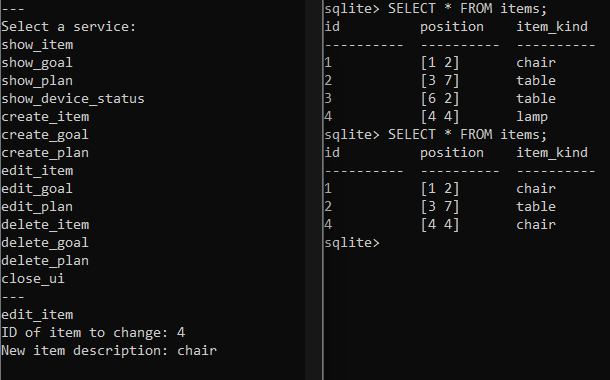
\includegraphics[width=(0.7\textwidth)]{Bilder/Eval1.png}
\caption{Evaluation: 'items' Datenbank}
\end{figure}

Im zweiten Schritt wird das Szenario angelegt. Hier werden zwei Szenarien angelegt. Das erste trägt die Beschreibung \dq set up a meeting \dq, hat als benötigte Gegenstände einen Tisch eingetragen und findet im Konferenzraum statt. Das zweite Szenario findet ebenfalls im Konferenzraum statt, trägt die Beschreibung \dq another meeting \dq und benötigt neben dem Tisch auch drei Stühle. Für diesen Test wird das zweite Szenario wieder gelöscht, und das erste wird so verändert, dass zwei Stühle zusätzlich zum Tisch benötigt werden.

\begin{figure}[h]
\centering
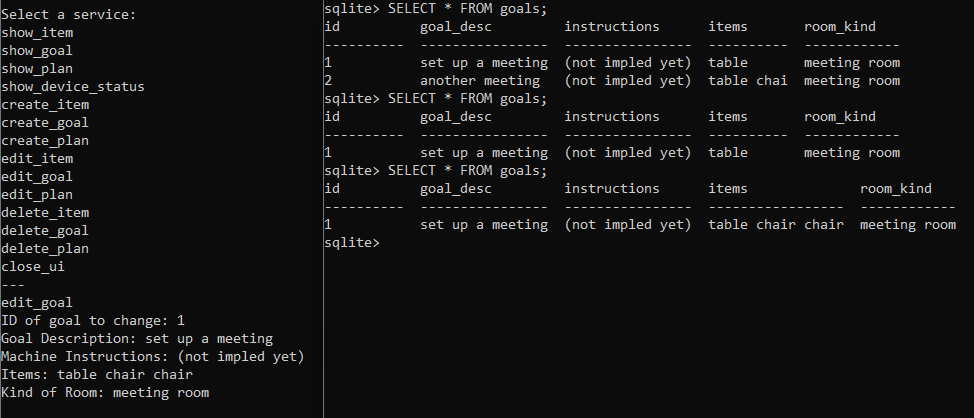
\includegraphics[width=(\textwidth)]{Bilder/Eval2.png}
\caption{Evaluation: 'goals' Datenbank}
\end{figure}

Im dritten und letzten Schritt wird das Szenario dann als Plan umgesetzt. Das aus dem letzten Schritt verbliebene Szenario besitzt die ID-Nummer 1, daher wird diese eingetragen. Statt der richtigen Uhrzeit wird aber Mitternacht des ersten Januar als Start-Zeitpunkt eingetragen und dementsprechend 1 Uhr nachts als End-Zeitpunkt. Ein zweiter Eintrag, der dasselbe Szenario umsetzen soll, erhält als Zeitpunkte 16, um sie visuell vom ersten Eintrag abzusetzen. Dieser zweiter Eintrag wird daraufhin wieder gelöscht, und die korrekte Zeiten 1672570800 und 1672574400, welche 12 und 13 Uhr mittags darstellen, werden im ersten Eintrag eingetragen. Dadurch liegt, wie in der Bildschirmaufnahme sichtbar, nur noch der korrekte Plan in der Datenbank.

\begin{figure}[h]
\centering
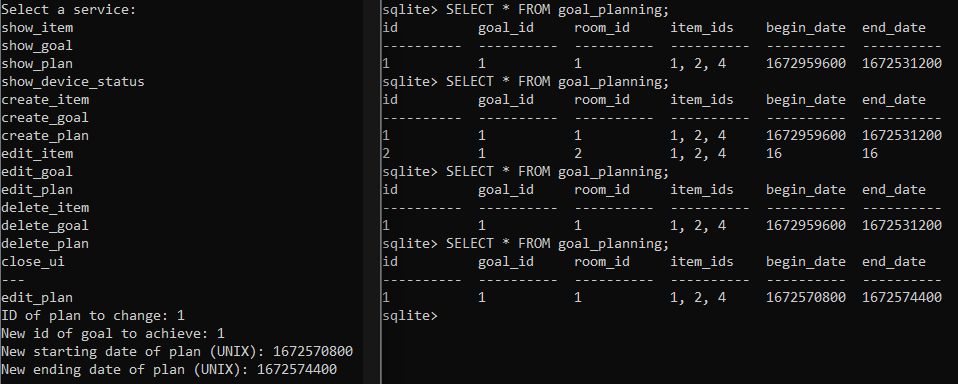
\includegraphics[width=(\textwidth)]{Bilder/Eval3.png}
\caption{Evaluation: 'goal\_planning' Datenbank}
\end{figure}

Durch das Anlegen eines Plans sollen auch Gegenstände reserviert werden, was wie im Ausschnitt unten erkennbar erfolgt. Der Eintrag 'item\_id' stimmt mit den im ersten Schritt angelegten Gegenständen überein, und die Zeiten sind ebenfalls der Änderung im dritten Schritt entsprechend. Demnach werden alle Funktionen wie erwartet ausgeführt.

\begin{figure}[h]
\centering
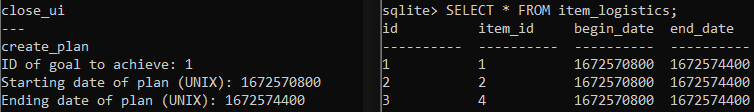
\includegraphics[width=(\textwidth)]{Bilder/Eval4.png}
\caption{Evaluation: 'item\_logistics' Datenbank}
\end{figure}
\setcounter{section}{0}

\addtocounter{chapter}{1}
\part{Diskussion\label{Diskussion}}
\section{Erfüllung der Anforderungen}

Die Implementierung, wie sie im vorherigen Kapitel beschrieben ist, legt den Grundstein für ein System, das allen gestellten Anforderungen gerecht werden kann. Um die Lücke zwischen den bisher erfüllten und gestellten Anforderungen zu schließen, ist jedoch noch weiterer Entwicklungsaufwand nötig. Das in Kapitel 3 gestellte Konzept, wenn wie beschrieben entwickelt, ist jedoch in der Lage, diese Lücke zu schließen.

Die Implementierung stellt vor allem die Grundlage dar, auf der die aufwendiger zu entwickelnden Funktionen aufbauen können. So ist die Eingabe von Nutzeranweisungen durch eine Konsoleneingabe mittels des User Interface-Knotens umgesetzt. Die dazu verwendete Funktion 'select\_service' ist dadurch, dass sie die Eingabe in einen Funktionsaufruf umwandelt, auch in der Lage, jede beliebige später hinzugefügte Aktion des Systems zu unterstützen, wenn diese im Knoten vorliegt. Auch die Status-Anzeige liegt in der Form des NodeUIOutput in einer Form vor, die alle bestehenden Aktionen abdeckt und sich beliebig erweitern lässt, um später hinzugefügte Funktionalitäten abzudecken.

Die Möglichkeit, Szenarien und Voreinstellungen zu erstellen, ist durch den Planungsknoten umgesetzt. Die Funktionen 'create\_goal' und 'create\_plan' ermöglichen es einem Nutzer, Szenarien zu erstellen und diese auch vom Knoten in einen Plan zusammenzufügen, falls dies logistisch möglich ist. Die Erstellung von sich wiederholenden Plänen muss in der derzeitigen Implementierung noch händisch erfolgen, die Schnittstelle ist aber so ausgelegt, dass eine Nutzeroberfläche bei einer Planung an sich wiederholenden Terminen diese parallel anfordern kann. Da die Knoten so angelegt sind, dass gleichzeitige Serviceanfragen jeweils einzelne Kommunikationsknoten öffnen, können diese parallel bearbeitet werden und ermöglichen so auch das Anlegen von mehreren Plänen gleichzeitig, sofern die Nutzeranwendung dies erlaubt.

Die Verständlichkeit der Semantik der Nutzereingabe wird dadurch gewährleistet, dass komplexe Prozesse, wie die Reservierung von Gegenständen für Pläne, im Hintergrund erfolgen, sodass nur selbsterklärende Eingaben erforderlich sind, welche nacheinander angefragt werden können. Dadurch kann gleichzeitig sicher gestellt werden, dass die erforderliche Eingabe per Kommandozeile verständlich ist, während eine Erweiterung um eine umfassendere Nutzeroberfläche, die die erforderlichen Eingaben an den Knoten sendet, nahtlos möglich ist. Durch diese Kapselung der Nutzereingabe ist es auch möglich, den Zugang auf das System auf diese Schnittstelle zu beschränken, ohne Funktionalität zu verlieren. Dadurch, dass ROS2 Nachrichten zwischen Knoten verschlüsseln kann, ist das System auch vor unberechtigtem Zugriff geschützt, wenn Teile des Systems auf verschiedenen Komponenten eines Computernetzes ausgeführt werden, wie es bei mobilen Robotern der Fall ist.

\newpage
Eine weiterführende Implementierung des Konzepts darf selbstverständlich diese bereits erfüllten Anforderungen nicht brechen, während sie die noch ausstehenden Anforderungen erfüllen muss. Der zu entwickelnde Navigationsknoten, welcher die Steuerung der verbundenen Geräte erlaubt, muss in der Lage sein, wie die bestehenden Knoten für eine größere Anzahl an Zugriffen skalierbar zu sein. Dazu muss er auch weiterhin die Verwendung der gesicherten Schnittstellen nutzen und die durchgeführten Aktionen verständlich dem Nutzer mitteilen können. Dies ist bei Beibehaltung der bestehenden Kommunikationsschemata ohne weitere Entwicklungsanstrengungen möglich. 

Es wird davon ausgegangen, dass die größte Herausforderung dieses Moduls die autonome Steuerung anhand der Szenarien und Planungsdaten sein wird. Eine Anwendung der Prinzipien der Arbeiten von Reily et al. \cite{silentSwarm} und Yang et al. in \cite{2DPlan} ist in der Lage, einen weitestgehend autonomen Betrieb des Systems zu erlauben, der auch robust gegenüber den Änderungen von laufenden Plänen ist. Eine zentrale Forschungsaufgabe hierbei wird es sein, den sicheren Betrieb in menschlicher Umgebung zu garantieren.

Eine dedizierte Nutzeranwendung, welche Zugriff auf das System gewährt, kann die verbliebenen noch offenen Anforderungen erfüllen. Eine graphische Oberfläche, welche den Prinzipien moderner nutzerzentrierten Designs folgt, kann die Eingabe der Nutzeranweisungen auch für Laien und Erstnutzer zugänglich machen. Hierbei wird weniger Forschungsarbeit als bei der Entwicklung der Navigation erwartet, da die Entwicklung von Nutzeroberflächen als weitgehend erforscht gilt und die benötigten Rahmenbedingungen durch das System bereits gegeben sind. Dabei muss auch hier darauf geachtet werden, dass die bereits etablierten gesicherten Kommunikationsschnittstellen verwendet werden, falls die Nutzeranwendung keine eigenen verwendet. In beiden Fällen muss darauf geachtet werden, dass ein Multi-User Konzept entwickelt wird, das die Verwendung durch Lehrende, Studenten und Administratoren unterstützt.


\newpage  \section{Implementierungsstrategie}

\subsection{Technische Voraussetzungen}

%Server
Um das konzeptionierte System in der Praxis zu verwenden, muss das Skills Lab einige Anforderungen über den üblichen Rahmen hinaus erfüllen. Zuerst ist ein zentraler Server nötig, auf dem es betrieben werden kann. Dabei muss jedoch keine unüblich große Leistung zur Verfügung stehen. Das System muss keine harten Echtzeit-Anforderungen erfüllen, solange die Rechenzeit von Operationen in einem für die Nutzer akzeptablen Rahmen liegen, da alle Prozesse asynchron stattfinden können.

%Internet
Grundvoraussetzung für die Verwendung von mobilen Roboterplattformen ist die Verfügbarkeit eines kabellosen Netzwerks, über das sich die Plattformen mit dem System verbinden können. Dies ist notwendig, um Anweisungen zu erhalten und Statusmeldungen senden zu können. Primär wäre hierfür ein WLAN-Netzwerk geeignet, da dieses eine universelle Kommunikation aller verwendeten Geräte ermöglicht. Durch den geplanten dezentralen Ansatz in der Navigation, in dem die Wegführung auf dem Roboter selbst stattfindet, muss dabei keine vollständige Abdeckung des Skills Labs mit einem Funknetzwerk erreicht werden. Je besser die Funkabdeckung des Skills Labs ist, desto höher ist die Erreichbarkeit von Plattformen und desto besser ist dementsprechend die Möglichkeit für das System, laufende Prozesse zu überwachen.

%Türen und Schwellen
Zusätzlich zu einem verfügbaren Netzwerkzugang müssen die Räume des Skills Labs so aufgebaut sein, dass Roboter sich in diesem frei bewegen können. Hierzu ist besonders der Zugang zu den verschiedenen Räumen wichtig. Da der überwältigende Anteil mobiler Roboter sich auf Rädern fortbewegt, ist das Vermeiden von Schwellen unabdingbar. Dazu müssen Türrahmen hoch und breit genug sein, damit sich die verwendeten Roboter und die zu transportierenden Möbel ohne Schwierigkeiten hindurch bewegen können. Bei der Verwendung von Türen ist es zudem wichtig, dass diese entweder zu Betriebszeiten offen stehen oder sich automatisch öffnen lassen, damit ein Zugang ohne Begleitung von Menschen möglich ist.

%Lageplan
Um den in der Implementierung verwendeten Koordinaten für Gegenstände und Roboter einen Kontext zu geben, muss eine digitale Karte des Skills Labs im Navigationsknoten vorliegen. Die Annahme ist, dass diese Navigationskarte über ein Koordinaten-Netz mit x- und y-Koordinaten verfügt, sodass die Position aller relevanten Bestandteile eindeutig beschrieben werden kann. Dazu zählen insbesondere Gegenstände, zu denen Roboter navigieren können müssen, sowie Positionen in den Simulationsräumen, an denen die Gegenstände platziert werden müssen. In der bisherigen Konzeptionierung wird von einer statischen Karte ausgegangen, welche nicht Personen oder mobile Möbelstücke umfasst.


\subsection{Aufwandsabschätzung}

%Vorwort
Bis zu einer vollständigen Implementierbarkeit des Systems sind neben der Erfüllung der technischen Voraussetzungen noch einige Schritte notwendig. Als Teil der Entwicklung der Navigations- und Nutzerschnittstellen, welche bereits beschrieben wurden, muss eine Nutzer- und Umgebungsevaluation durchgeführt werden, um die fehlenden Komponenten genau an die Skills Labs, welche diese verwenden sollen, anzupassen. Aus dieser kann auch erst eine genaue Aufstellung des Arbeitsaufwands der benötigten Komponenten erstellt werden, jedoch kann bereits eine ungefähre Einordnung erfolgen.

%Navigation
Die Entwicklung des Navigationsknotens und der dazugehörigen Algorithmen stellt aller Voraussicht nach den Inhalt einer weiteren Forschungsarbeit dar. Die Arbeiten von Reily et al. \cite{silentSwarm}, Yang et al. \cite{2DPlan} und De La Puente et al. \cite{assistRobot} geben einen plausiblen Forschungsansatz vor, wurden bisher aber nicht in einem gemeinsamen Algorithmus verwendet. Auch gilt es, die Schnittstelle zur Verbindung mit dem System zu programmieren.

%Installation
Die Inbetriebnahme des restlichen Systems auf einem bestehenden Server stellt dagegen einen vergleichsweise vernachlässigbaren Aufwand dar. Da ROS2 auf den verbreitetsten Betriebssystemen betrieben werden kann und SQLite über Python gleichermaßen auf nahezu allen Plattformen unterstützt wird, kann davon ausgegangen werden, dass die Installation ohne weitere Anpassungen erfolgen kann. Je nach Wahl und der Verfügbarkeit von Roboterplattformen kann hier der Aufwand jedoch höher sein.

%Roboter-Einbindung
Da das Robot Operating System in seiner zweiten Version im Vergleich zu ROS1 relativ jung ist, ist die Zahl der nativ unterstützten Roboter auch vergleichsweise gering. Plattformen, die nur die erste Version des Frameworks unterstützen, können durch eine Übersetzungsschnittstelle in ROS2 verwendet werden, dies ist jedoch mit zusätzlichem Aufwand verbunden. Die Einbindung von Robotern, welche keine der beiden Versionen der Framework unterstützen, stellt sich erfahrungsgemäß als möglich, aber sehr aufwendig heraus. Hier müsste eine eigene Schnittstelle für den Roboter entwickelt werden, welche die ROS-Anweisungen in das vom Roboter unterstützten, und die Daten des Roboters zurück in ein vom System verstandenes Format übersetzt.

%Training
Zuletzt muss auch das Training der Nutzer in Betracht gezogen werden. Da das System dafür konzipiert ist, primär von Lehrenden und Betreuern verwendet zu werden, muss sicher gestellt werden, dass diese es auch voll ausschöpfen können. Dazu müssen Schulungen oder Informationsmaterial zur Verfügung gestellt werden, welche im Rahmen der Nutzerschnittstellen-Entwicklung erstellt werden müssen. Zusätzlich zu den Nutzern benötigt das System auch Administratoren, welche das System warten und verwalten können. Da dies sowohl Software- als auch spezialisierte Hardware-Komponenten in Form von Roboterplattformen umfasst, ist das Training dieser dementsprechend aufwendiger.


\section{Implementierung in Skills Labs}

Die Umsetzung des Konzepts in der Praxis kann sich als aufwendig oder gar unmöglich herausstellen, falls die technischen Herausforderungen in einer bestehenden Einrichtung nicht gegeben sind. Während Komponenten, wie eine Abdeckung durch ein Funknetzwerk, vergleichsweise leicht nachrüstbar sind, sind bauliche Einschränkungen schwerer zu beheben. Bestehende Türrahmen, welche über Schwellen oder zu geringe Breiten verfügen, sind kostspielig zu ersetzen. Auch eine komplett fehlende IT-Infrastruktur nachträglich zu verbauen stellt unter Umständen eine zu große Investition dar, um die Kosten- und Arbeitsersparnis zu rechtfertigen. Eine zentrale Voraussetzung ist auch das Vorhandensein eines Lagers, aus welchem die Simulationsräume bestückt werden können. Dieses benötigt eine gewisse Größe und Zugänglichkeit, welche nicht unbedingt durch bestehende Mehrzweck-Räume abgedeckt werden kann.

Bei der Planung von neuen Skills Labs sind diese Voraussetzungen ungleich einfacher zu erfüllen, da viele der Voraussetzungen keinen großen Mehraufwand bei der Planung darstellen. Die Einbindung von WLAN-Netzen wird in Neubauten als üblich angesehen, da von der Verwendung von Computersystemen in der Lehre ausgegangen werden kann. Auch ist die Bereitstellung eines Lagers während der Planung eines Gebäudes wesentlich einfacher umzusetzen als bei einer Nachrüstung.

Eine Gebäudeplanung nach DIN 18040-1, welche die Gestaltung von öffentlich zugänglichen Gebäuden beschreibt, erfüllt auch die baulichen Voraussetzungen für die Verwendung von Roboterplattformen. Insbesondere die Mindestgröße von Türrahmen, die ausreichende Bewegungsfläche vor Zugängen und die Abwesenheit von Türschwellen spielen hier zentrale Rollen. Auch wird in öffentlichen Gebäuden ohnehin gefordert, dass Türen sich automatisch öffnen lassen, sodass eine Einbindung in ein elektronisches System nur einen geringen Mehraufwand darstellt.

Die Auswahl von Roboterplattformen ist hauptsächlich von den Anforderungen der gegebenen Aufgaben abhängig, daher kann hier keine allgemeine Abschätzung erfolgen. Für den Transport von Möbeln, wie Liegen und Tischen, werden beispielsweise Plattformen, die einem Gabelstapler ähneln können, verwendet, während der Transport von Abfalleimern und kleinen Simulatoren und Verbrauchsgegenständen eine Plattform ähnlich einem Rollwagen bevorzugen würde. Die Wahl und eventuelle Entwicklung der Plattformen sollte daher abhängig von allen anderen Faktoren geschehen.


\newpage \section{Reflektion}

Das Projekt hat sich während der Arbeit daran als umfangreicher als initial erwartet herausgestellt. Es ist von vornherein davon ausgegangen worden, dass die Navigation einen großen Teil des Systems darstellen wird, jedoch wurde in der Projektplanung davon ausgegangen, dass diese im Rahmen dieser Forschungsarbeit implementiert werden kann. Während der Recherchearbeit hat sich allerdings herausgestellt, dass die Entwicklung des Frameworks des Systems allein schon den Umfang der Arbeit ausfüllt. Da dementsprechend die Inbetriebnahme des Systems zum Zeitpunkt dieses Berichts aber nicht möglich ist, kann die Forschungsfrage nur als teilweise beantwortet betrachtet werden.

Die Verwendung von ROS als Grundlage für das System wurde schon in der Vorbereitungsphase als beste verfügbare open-source Lösung identifiziert. Die Implementierung bewies, dass das Framework gut für den gewählten Ansatz geeignet ist und alle Anforderungen erfüllen kann. Die Verwendung von SQLite und Python erwies sich als gleichermaßen erfolgreich, auch wenn es hier viele genauso geeignete Lösungen gegeben hat und der Auswahl keine besondere Bedeutung für das Gesamtkonzept zugesprochen wird. Die Auswahl an Werkzeugen erscheint dementsprechend gelungen.

Die Experten-Interviews während der Recherche haben eine interessante Perspektive des derzeitigen Standes der Automation in Skills Labs aufgezeigt. Es ist initial davon ausgegangen worden, dass bereits ein höherer Grad der Einbindung von technischen Systemen vorhanden ist und auf diesen aufgebaut werden kann. Auch die Diversität der Voraussetzungen und Möglichkeiten der verschiedenen Skills Labs erwies sich als größer als vormals angenommen. Dementsprechend wird es als sehr positiv angesehen, dass sie in dieser Form durchgeführt wurden, da so die Bedeutung eines möglichst universell einsetzbaren und einfach zu implementierbaren Systems identifiziert werden konnte. Dementsprechend wird die Recherche als sehr erfolgreich und impulsgebend betrachtet.

Insgesamt kann die Arbeit als Erfolg betrachtet werden. Auch wenn das eingangs gestellte Ziel eines betriebsbereiten Automationssystems nicht vollständig erreicht wurde, wurden wertvolle Erkenntnisse zusammengetragen und eine umfassende Grundlage gelegt. Es ist gelungen, einen realistischen Ausblick auf die Möglichkeiten und Anforderungen eines solchen Systems darzustellen. Dadurch wird Skills Labs die Möglichkeit gegeben, eine informierte Entscheidung über eine Weiterverfolgung dieses Ansatzes zu treffen.
\setcounter{section}{0}

\addtocounter{chapter}{1}
\part{Fazit\label{Fazit}}
\section{Zusammenfassung}

In dieser Arbeit wurde die Forschungsaufgabe bearbeitet, ein Konzept für die Automatisierung von Skills Labs mithilfe von mobilen Robotern zu entwickeln. Dies ist auf Grundlage von Experteninterviews und einer Literaturrecherche erfolgt, welche die Anforderungen des Konzepts vorgegeben haben.

Es wurde identifiziert, dass ein solches Automationssystem in der Lage sein muss, sich mit Geräten wie mobilen Robotern zu verbinden und an diese Befehle zu geben, die den Anweisungen der Nutzer entsprechen. Dazu sollen die Nutzer in der Lage sein, Szenarien zu erstellen, die vom System autonom umgesetzt werden, ohne dass die Roboter von Menschen überwacht werden müssen. Damit dies reibungslos funktioniert, muss es ein Multi-User Konzept geben, welches den Zugriff von mehreren Nutzern ohne die Entstehung von Kollisionen erlaubt.

Auf Grundlage dieser Anforderungen wurde ein Konzept entwickelt, welches um die vier Eckpfeiler User Interface, Logistik, Planung und Navigation herum aufgebaut ist. Das User Interface nimmt die Anweisungen der Nutzer entgegen und zeigt Statusmeldungen des Systems an. Die Logistik verwaltet den Bestand an Gegenständen und Möbeln, welche in den Szenarien verwendet werden. Die Planung verwaltet im Gegenzug die Szenarien selbst und plant die Ausführung dieser. Dazu weist sie auch die Logistik an, Gegenstände zu reservieren, damit diese zum Ausführungszeitpunkt verfügbar sind. Die Navigation schließlich ist für die Ausführung dieser Szenarien verantwortlich. Sie kommuniziert mit den Robotern und gibt ihnen Navigationsanweisungen, um die Szenarien in der Praxis umzusetzen.

Basierend auf dem Konzept wurde dann ein Prototyp des Systems gebaut, um die Machbarkeit zu belegen. Dieser umfasst die ersten drei Eckpfeiler, welche die nutzerseitigen Teile des Systems bilden. Es wurde gezeigt, dass ein solches System im Rahmen der gestellten Anforderungen auch mit begrenzten Ressourcen umsetzbar ist. Es wurde allerdings auch festgestellt, dass die Implementierung der Navigation einen größeren Arbeitsaufwand erfordert, als im Rahmen dieser Bachelorarbeit umgesetzt werden kann.

In einer abschließenden Diskussion wurden die zur Implementierung nötigen Schritte festgestellt. Es wurde dargestellt, welche Komponenten noch zu einer Ausführung in der Praxis fehlen und wie diese entwickelt werden können. Dabei wurden die Herausforderungen einer Implementierung in neu gebauten und bestehenden Skills Labs identifiziert und ein Ausblick auf eine Weiterentwicklung des Konzepts gegeben.

\newpage \section{Ausblick}

Die hier vorgestellte Arbeit stellt einen Wegplan für das vorgestellte System dar. Für eine Verwendung des Systems in der Praxis ist weitere Forschungs- und Entwicklungsarbeit vonnöten. Primär muss ein Algorithmus zur Ausführung der Navigation entwickelt werden. Die vorgestellten Ansätze der derzeitigen Forschung bieten hierfür einen Einstiegspunkt an, während die noch nicht umgesetzten Anforderungen die Rahmenbedingungen stellen. Dazu muss eine Benutzeroberfläche entwickelt werden, welche das geforderte Multi-User Konzept umsetzt und einen ergonomischen Zugang zum System gewährt. Auch ist es wichtig, dass bei einer Implementierung in einem konkreten Skills Lab die Voraussetzungen und zu automatisierenden Aufgaben untersucht werden und eine Standort- und Nutzeranalyse durchgeführt wird. Dabei können insbesondere weitere Verwendungsmöglichkeiten des Systems erarbeitet werden, die über den Transport von Möbeln hinausgehen.

Das hier vorgestellte System soll daher nicht als fertige Lösung angesehen werden, sondern als Einstieg in das Forschungsfeld der Automation im Kontext der Life Science Lehre. Da bisher wenige Arbeiten auf diesem Feld durchgeführt wurden, gibt es viele noch nicht betrachtete Blickwinkel, aus denen dies beleuchtet werden kann. Die Modernisierung und Verwendung von digitalen Werkzeugen in der Lehre wird vermutlich von immer größerer Bedeutung sein. Besonders bei der Ausbildung für die Verwendung von cyber-physikalischen Systemen, die in der Praxis von Bedeutung sind, kann die Integration von Automatismen in der Lehre helfen.

Dabei ist es jedoch wichtig, solche Systeme zu identifizieren, die einen echten Mehrwert bieten, um die Entwicklung dieser zu fördern. Da Automatisierung oft mit beträchtlichen Investitionen verbunden ist, ist die Erforschung von kosteneffizienten Lösungen eine zentrale Voraussetzung für die Akzeptanz solcher Werkzeuge. Die hier vorgestellte Arbeit setzt voraus, dass Roboterplattformen verfügbar sind oder angeschafft werden können. Je nach Aufgabe können diese Kosten verursachen, die für Skills Labs nicht tragbar sind. Eine mögliche Forschungsaufgabe wäre neben der Entwicklung der Navigation also auch, kostengünstige Plattformen zu bauen, welche die Anforderungen erfüllen können, um nicht auf vorgefertigte Geräte zurückgreifen zu müssen.

Die vorgestellten Forschungsansätze, auf denen das System aufbaut, stellen nur einen kleinen Teil der aktuell entwickelten Projekte dar. Ein großer Teil der Automatisierungsforschung ist extrem zweckgebunden, da sie in der Wirtschaft zur Lösung spezifischer Probleme stattfindet. Die Erforschung von universellen Lösungen, auf denen in allen Bereichen des Lebens aufgebaut werden kann, sollte bei der Weiterentwicklung dieses Systems im Vordergrund stehen. Das hier vorgestellte Konzept kann, in einem größeren Maßstab, auch auf Warenhäuser in der Wirtschaft, Krankenhäuser und andere Arten des Unterrichts ausgeweitet werden, ohne den Kern des Konzepts zu verändern. Dementsprechend kann eine Weiterentwicklung auch in Anbetracht anderer Einsatzorte erfolgen, wo eine Automatisierung von Bedeutung sein kann.
\setcounter{section}{0}

\addtocounter{chapter}{1}
\part*{Anhang}
\appendix

\listoffigures % Abbildungsverzeichnis
\listoftables % Tabellenverzeichnis

%%% --------------------------------------------------
%%% Bibliographie
%%% --------------------------------------------------

% \addcontentsline{toc}{section}{Literaturverzeichnis}
%%% --------------------------------------------------
%%% Bibliographie
%%% --------------------------------------------------
%\renewcommand{\bibfont}{\scriptsize}
\printbibliography[title={Literaturverzeichnis}, heading=bibintoc]


%%% --------------------------------------------------
%%% Index
%%% --------------------------------------------------
{\setkomafont{chapter}{\Huge} % temporarily set chapter font
\printindex
}

\end{document}

%%% % dummy indices for page breaks in Index
%%% \index{GleichungrZZZ@{\hspace*{72ex}}|myNewpage}
%%% %\index{MaximalZZZ@{\hspace*{72ex}}|myNewpage}
%%% %\index{ZZZ@{\hspace*{72ex}}|myVspace{8cm}}
%%% \index{EZZZ@{\hspace*{72ex}}|myVspace{-1ex}}
%%% \index{Faaa@{\hspace*{72ex}}|myVspace{-1.5ex}}
%%% \index{FZZZ@{\hspace*{72ex}}|myVspace{-1.5ex}}
%%% \index{Gaaa@{\hspace*{72ex}}|myVspace{-1.5ex}}
%%% \index{LZZZ@{\hspace*{72ex}}|myVspace{-.3ex}}
%%% \index{Maaa@{\hspace*{72ex}}|myVspace{-.5ex}}


